\documentclass[1p]{elsarticle_modified}
%\bibliographystyle{elsarticle-num}

%\usepackage[colorlinks]{hyperref}
%\usepackage{abbrmath_seonhwa} %\Abb, \Ascr, \Acal ,\Abf, \Afrak
\usepackage{amsfonts}
\usepackage{amssymb}
\usepackage{amsmath}
\usepackage{amsthm}
\usepackage{scalefnt}
\usepackage{amsbsy}
\usepackage{kotex}
\usepackage{caption}
\usepackage{subfig}
\usepackage{color}
\usepackage{graphicx}
\usepackage{xcolor} %% white, black, red, green, blue, cyan, magenta, yellow
\usepackage{float}
\usepackage{setspace}
\usepackage{hyperref}

\usepackage{tikz}
\usetikzlibrary{arrows}

\usepackage{multirow}
\usepackage{array} % fixed length table
\usepackage{hhline}

%%%%%%%%%%%%%%%%%%%%%
\makeatletter
\renewcommand*\env@matrix[1][\arraystretch]{%
	\edef\arraystretch{#1}%
	\hskip -\arraycolsep
	\let\@ifnextchar\new@ifnextchar
	\array{*\c@MaxMatrixCols c}}
\makeatother %https://tex.stackexchange.com/questions/14071/how-can-i-increase-the-line-spacing-in-a-matrix
%%%%%%%%%%%%%%%

\usepackage[normalem]{ulem}

\newcommand{\msout}[1]{\ifmmode\text{\sout{\ensuremath{#1}}}\else\sout{#1}\fi}
%SOURCE: \msout is \stkout macro in https://tex.stackexchange.com/questions/20609/strikeout-in-math-mode

\newcommand{\cancel}[1]{
	\ifmmode
	{\color{red}\msout{#1}}
	\else
	{\color{red}\sout{#1}}
	\fi
}

\newcommand{\add}[1]{
	{\color{blue}\uwave{#1}}
}

\newcommand{\replace}[2]{
	\ifmmode
	{\color{red}\msout{#1}}{\color{blue}\uwave{#2}}
	\else
	{\color{red}\sout{#1}}{\color{blue}\uwave{#2}}
	\fi
}

\newcommand{\Sol}{\mathcal{S}} %segment
\newcommand{\D}{D} %diagram
\newcommand{\A}{\mathcal{A}} %arc


%%%%%%%%%%%%%%%%%%%%%%%%%%%%%5 test

\def\sl{\operatorname{\textup{SL}}(2,\Cbb)}
\def\psl{\operatorname{\textup{PSL}}(2,\Cbb)}
\def\quan{\mkern 1mu \triangleright \mkern 1mu}

\theoremstyle{definition}
\newtheorem{thm}{Theorem}[section]
\newtheorem{prop}[thm]{Proposition}
\newtheorem{lem}[thm]{Lemma}
\newtheorem{ques}[thm]{Question}
\newtheorem{cor}[thm]{Corollary}
\newtheorem{defn}[thm]{Definition}
\newtheorem{exam}[thm]{Example}
\newtheorem{rmk}[thm]{Remark}
\newtheorem{alg}[thm]{Algorithm}

\newcommand{\I}{\sqrt{-1}}
\begin{document}

%\begin{frontmatter}
%
%\title{Boundary parabolic representations of knots up to 8 crossings}
%
%%% Group authors per affiliation:
%\author{Yunhi Cho} 
%\address{Department of Mathematics, University of Seoul, Seoul, Korea}
%\ead{yhcho@uos.ac.kr}
%
%
%\author{Seonhwa Kim} %\fnref{s_kim}}
%\address{Center for Geometry and Physics, Institute for Basic Science, Pohang, 37673, Korea}
%\ead{ryeona17@ibs.re.kr}
%
%\author{Hyuk Kim}
%\address{Department of Mathematical Sciences, Seoul National University, Seoul 08826, Korea}
%\ead{hyukkim@snu.ac.kr}
%
%\author{Seokbeom Yoon}
%\address{Department of Mathematical Sciences, Seoul National University, Seoul, 08826,  Korea}
%\ead{sbyoon15@snu.ac.kr}
%
%\begin{abstract}
%We find all boundary parabolic representation of knots up to 8 crossings.
%
%\end{abstract}
%\begin{keyword}
%    \MSC[2010] 57M25 
%\end{keyword}
%
%\end{frontmatter}

%\linenumbers
%\tableofcontents
%
\newcommand\colored[1]{\textcolor{white}{\rule[-0.35ex]{0.8em}{1.4ex}}\kern-0.8em\color{red} #1}%
%\newcommand\colored[1]{\textcolor{white}{ #1}\kern-2.17ex	\textcolor{white}{ #1}\kern-1.81ex	\textcolor{white}{ #1}\kern-2.15ex\color{red}#1	}

{\Large $\underline{12a_{0419}~(K12a_{0419})}$}

\setlength{\tabcolsep}{10pt}
\renewcommand{\arraystretch}{1.6}
\vspace{1cm}\begin{tabular}{m{100pt}>{\centering\arraybackslash}m{274pt}}
\multirow{5}{120pt}{
	\centering
	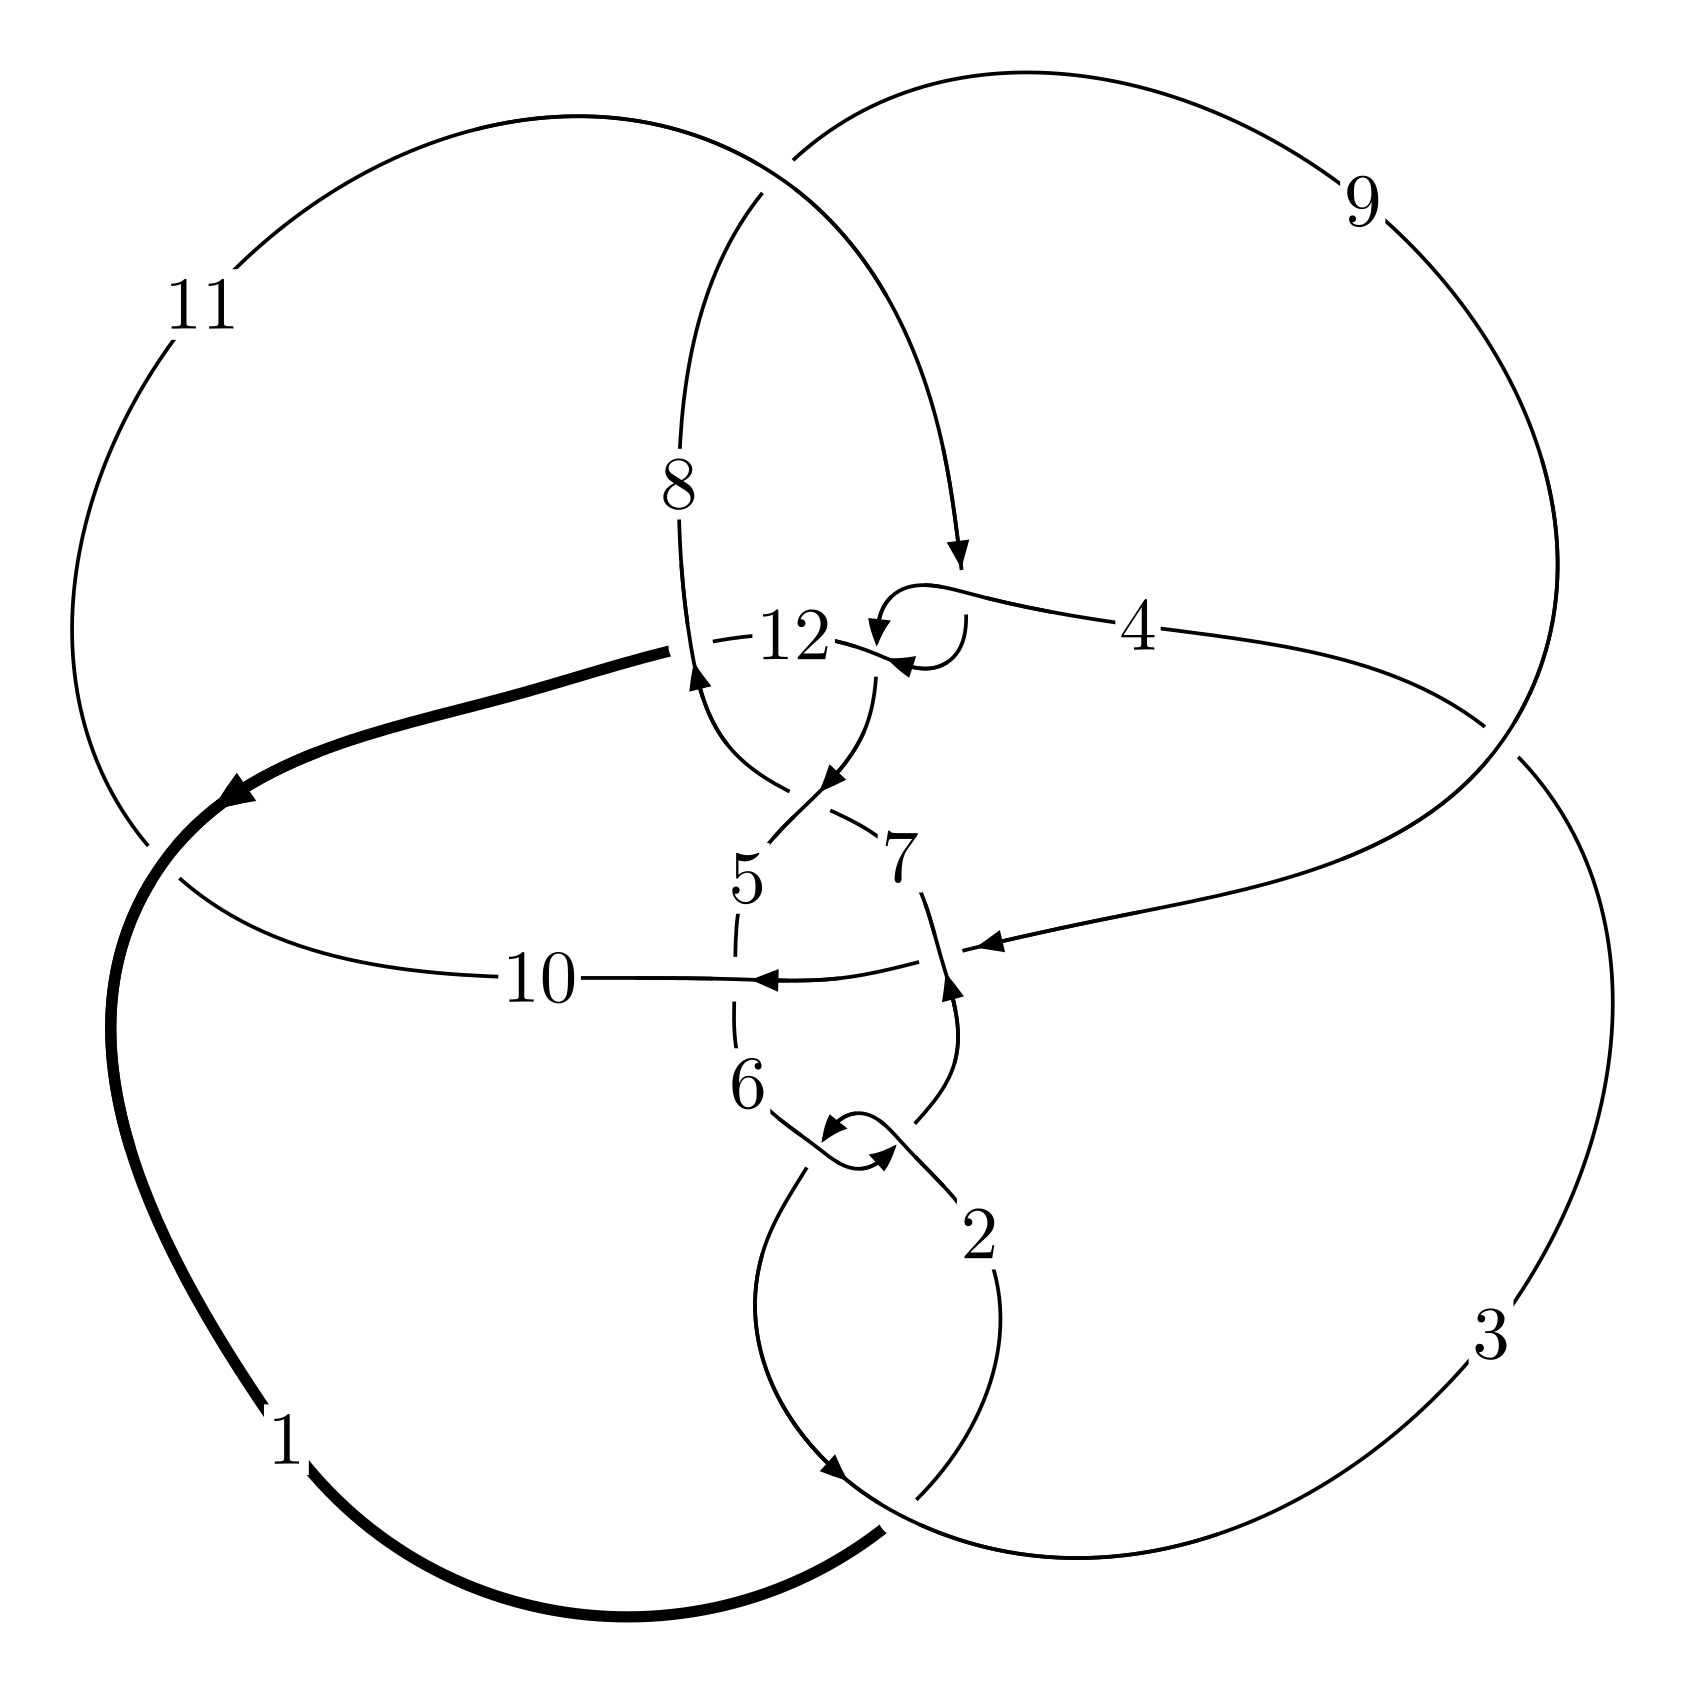
\includegraphics[width=112pt]{../../../GIT/diagram.site/Diagrams/png/1220_12a_0419.png}\\
\ \ \ A knot diagram\footnotemark}&
\allowdisplaybreaks
\textbf{Linearized knot diagam} \\
\cline{2-2}
 &
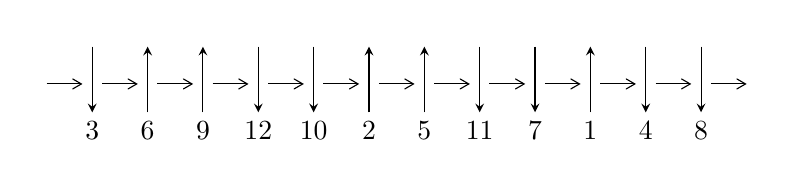
\begin{tikzpicture}[x=20pt, y=17pt]
	% nodes
	\node (C0) at (0, 0) {};
	\node (C1) at (1, 0) {};
	\node (C1U) at (1, +1) {};
	\node (C1D) at (1, -1) {3};

	\node (C2) at (2, 0) {};
	\node (C2U) at (2, +1) {};
	\node (C2D) at (2, -1) {6};

	\node (C3) at (3, 0) {};
	\node (C3U) at (3, +1) {};
	\node (C3D) at (3, -1) {9};

	\node (C4) at (4, 0) {};
	\node (C4U) at (4, +1) {};
	\node (C4D) at (4, -1) {12};

	\node (C5) at (5, 0) {};
	\node (C5U) at (5, +1) {};
	\node (C5D) at (5, -1) {10};

	\node (C6) at (6, 0) {};
	\node (C6U) at (6, +1) {};
	\node (C6D) at (6, -1) {2};

	\node (C7) at (7, 0) {};
	\node (C7U) at (7, +1) {};
	\node (C7D) at (7, -1) {5};

	\node (C8) at (8, 0) {};
	\node (C8U) at (8, +1) {};
	\node (C8D) at (8, -1) {11};

	\node (C9) at (9, 0) {};
	\node (C9U) at (9, +1) {};
	\node (C9D) at (9, -1) {7};

	\node (C10) at (10, 0) {};
	\node (C10U) at (10, +1) {};
	\node (C10D) at (10, -1) {1};

	\node (C11) at (11, 0) {};
	\node (C11U) at (11, +1) {};
	\node (C11D) at (11, -1) {4};

	\node (C12) at (12, 0) {};
	\node (C12U) at (12, +1) {};
	\node (C12D) at (12, -1) {8};
	\node (C13) at (13, 0) {};

	% arrows
	\draw[->,>={angle 60}]
	(C0) edge (C1) (C1) edge (C2) (C2) edge (C3) (C3) edge (C4) (C4) edge (C5) (C5) edge (C6) (C6) edge (C7) (C7) edge (C8) (C8) edge (C9) (C9) edge (C10) (C10) edge (C11) (C11) edge (C12) (C12) edge (C13) ;	\draw[->,>=stealth]
	(C1U) edge (C1D) (C2D) edge (C2U) (C3D) edge (C3U) (C4U) edge (C4D) (C5U) edge (C5D) (C6D) edge (C6U) (C7D) edge (C7U) (C8U) edge (C8D) (C9U) edge (C9D) (C10D) edge (C10U) (C11U) edge (C11D) (C12U) edge (C12D) ;
	\end{tikzpicture} \\
\hhline{~~} \\& 
\textbf{Solving Sequence} \\ \cline{2-2} 
 &
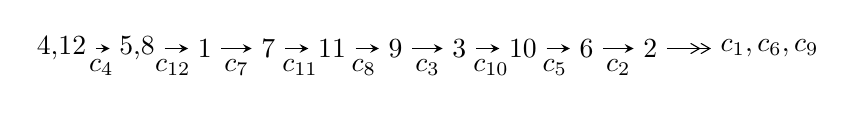
\begin{tikzpicture}[x=23pt, y=7pt]
	% node
	\node (A0) at (-1/8, 0) {4,12};
	\node (A1) at (17/16, 0) {5,8};
	\node (A2) at (17/8, 0) {1};
	\node (A3) at (25/8, 0) {7};
	\node (A4) at (33/8, 0) {11};
	\node (A5) at (41/8, 0) {9};
	\node (A6) at (49/8, 0) {3};
	\node (A7) at (57/8, 0) {10};
	\node (A8) at (65/8, 0) {6};
	\node (A9) at (73/8, 0) {2};
	\node (C1) at (1/2, -1) {$c_{4}$};
	\node (C2) at (13/8, -1) {$c_{12}$};
	\node (C3) at (21/8, -1) {$c_{7}$};
	\node (C4) at (29/8, -1) {$c_{11}$};
	\node (C5) at (37/8, -1) {$c_{8}$};
	\node (C6) at (45/8, -1) {$c_{3}$};
	\node (C7) at (53/8, -1) {$c_{10}$};
	\node (C8) at (61/8, -1) {$c_{5}$};
	\node (C9) at (69/8, -1) {$c_{2}$};
	\node (A10) at (11, 0) {$c_{1},c_{6},c_{9}$};

	% edge
	\draw[->,>=stealth]	
	(A0) edge (A1) (A1) edge (A2) (A2) edge (A3) (A3) edge (A4) (A4) edge (A5) (A5) edge (A6) (A6) edge (A7) (A7) edge (A8) (A8) edge (A9) ;
	\draw[->>,>={angle 60}]	
	(A9) edge (A10);
\end{tikzpicture} \\ 

\end{tabular} \\

\footnotetext{
The image of knot diagram is generated by the software ``\textbf{Draw programme}" developed by Andrew Bartholomew(\url{http://www.layer8.co.uk/maths/draw/index.htm\#Running-draw}), where we modified some parts for our purpose(\url{https://github.com/CATsTAILs/LinksPainter}).
}\phantom \\ \newline 
\centering \textbf{Ideals for irreducible components\footnotemark of $X_{\text{par}}$} 
 
\begin{align*}
I^u_{1}&=\langle 
9.88459\times10^{1013} u^{181}+1.80208\times10^{1014} u^{180}+\cdots+2.42399\times10^{1014} b+3.99849\times10^{1014},\\
\phantom{I^u_{1}}&\phantom{= \langle  }-2.88553\times10^{1013} u^{181}-4.79670\times10^{1013} u^{180}+\cdots+1.27578\times10^{1013} a-1.17798\times10^{1014},\\
\phantom{I^u_{1}}&\phantom{= \langle  }u^{182}+2 u^{181}+\cdots+18 u+1\rangle \\
I^u_{2}&=\langle 
-1.15838\times10^{33} u^{42}-1.70244\times10^{33} u^{41}+\cdots+2.11466\times10^{32} b-1.33001\times10^{33},\\
\phantom{I^u_{2}}&\phantom{= \langle  }-1.28770\times10^{33} u^{42}+1.62157\times10^{32} u^{41}+\cdots+2.11466\times10^{32} a-6.36585\times10^{33},\;u^{43}+u^{42}+\cdots+2 u+1\rangle \\
\\
\end{align*}
\raggedright * 2 irreducible components of $\dim_{\mathbb{C}}=0$, with total 225 representations.\\
\footnotetext{All coefficients of polynomials are rational numbers. But the coefficients are sometimes approximated in decimal forms when there is not enough margin.}
\newpage
\renewcommand{\arraystretch}{1}
\centering \section*{I. $I^u_{1}= \langle 9.88\times10^{1013} u^{181}+1.80\times10^{1014} u^{180}+\cdots+2.42\times10^{1014} b+4.00\times10^{1014},\;-2.89\times10^{1013} u^{181}-4.80\times10^{1013} u^{180}+\cdots+1.28\times10^{1013} a-1.18\times10^{1014},\;u^{182}+2 u^{181}+\cdots+18 u+1 \rangle$}
\flushleft \textbf{(i) Arc colorings}\\
\begin{tabular}{m{7pt} m{180pt} m{7pt} m{180pt} }
\flushright $a_{4}=$&$\begin{pmatrix}1\\0\end{pmatrix}$ \\
\flushright $a_{12}=$&$\begin{pmatrix}0\\u\end{pmatrix}$ \\
\flushright $a_{5}=$&$\begin{pmatrix}1\\u^2\end{pmatrix}$ \\
\flushright $a_{8}=$&$\begin{pmatrix}2.26177 u^{181}+3.75981 u^{180}+\cdots+147.770 u+9.23341\\-0.407782 u^{181}-0.743438 u^{180}+\cdots-27.0959 u-1.64955\end{pmatrix}$ \\
\flushright $a_{1}=$&$\begin{pmatrix}-3.27635 u^{181}-5.34779 u^{180}+\cdots-141.246 u-8.30418\\-0.0374048 u^{181}+0.441289 u^{180}+\cdots+39.6804 u+3.60649\end{pmatrix}$ \\
\flushright $a_{7}=$&$\begin{pmatrix}3.24310 u^{181}+4.95955 u^{180}+\cdots+186.351 u+11.6467\\0.352908 u^{181}-0.162965 u^{180}+\cdots-14.3448 u-0.886637\end{pmatrix}$ \\
\flushright $a_{11}=$&$\begin{pmatrix}u\\u\end{pmatrix}$ \\
\flushright $a_{9}=$&$\begin{pmatrix}2.89776 u^{181}+4.31013 u^{180}+\cdots+160.146 u+10.0693\\0.228210 u^{181}-0.193110 u^{180}+\cdots-14.7200 u-0.813692\end{pmatrix}$ \\
\flushright $a_{3}=$&$\begin{pmatrix}3.44546 u^{181}+6.53680 u^{180}+\cdots+327.617 u+24.9418\\-0.447829 u^{181}-0.305439 u^{180}+\cdots+2.78794 u+0.556196\end{pmatrix}$ \\
\flushright $a_{10}=$&$\begin{pmatrix}-4.22856 u^{181}-7.89659 u^{180}+\cdots-295.726 u-32.9946\\0.193692 u^{181}+0.370684 u^{180}+\cdots+18.9442 u+1.19168\end{pmatrix}$ \\
\flushright $a_{6}=$&$\begin{pmatrix}-5.48557 u^{181}-10.1286 u^{180}+\cdots-548.088 u-44.6091\\-0.455170 u^{181}-0.262679 u^{180}+\cdots-12.6569 u-1.01401\end{pmatrix}$ \\
\flushright $a_{2}=$&$\begin{pmatrix}-1.47936 u^{181}-3.47355 u^{180}+\cdots-84.2762 u-8.47404\\0.452183 u^{181}+0.416483 u^{180}+\cdots+37.1423 u+2.46176\end{pmatrix}$\\&\end{tabular}
\flushleft \textbf{(ii) Obstruction class $= -1$}\\~\\
\flushleft \textbf{(iii) Cusp Shapes $= -1.74311 u^{181}-3.28687 u^{180}+\cdots-161.807 u-22.4706$}\\~\\
\newpage\renewcommand{\arraystretch}{1}
\flushleft \textbf{(iv) u-Polynomials at the component}\newline \\
\begin{tabular}{m{50pt}|m{274pt}}
Crossings & \hspace{64pt}u-Polynomials at each crossing \\
\hline $$\begin{aligned}c_{1}\end{aligned}$$&$\begin{aligned}
&u^{182}+80 u^{181}+\cdots-14 u+1
\end{aligned}$\\
\hline $$\begin{aligned}c_{2},c_{6}\end{aligned}$$&$\begin{aligned}
&u^{182}+40 u^{180}+\cdots+4 u+1
\end{aligned}$\\
\hline $$\begin{aligned}c_{3}\end{aligned}$$&$\begin{aligned}
&u^{182}+u^{181}+\cdots+173061562687 u+50838216514
\end{aligned}$\\
\hline $$\begin{aligned}c_{4},c_{11}\end{aligned}$$&$\begin{aligned}
&u^{182}+2 u^{181}+\cdots+18 u+1
\end{aligned}$\\
\hline $$\begin{aligned}c_{5}\end{aligned}$$&$\begin{aligned}
&u^{182}-6 u^{180}+\cdots-29 u+1
\end{aligned}$\\
\hline $$\begin{aligned}c_{7}\end{aligned}$$&$\begin{aligned}
&u^{182}+16 u^{181}+\cdots+107815334379 u+9487345129
\end{aligned}$\\
\hline $$\begin{aligned}c_{8}\end{aligned}$$&$\begin{aligned}
&u^{182}+18 u^{181}+\cdots+37740592 u+2302703
\end{aligned}$\\
\hline $$\begin{aligned}c_{9}\end{aligned}$$&$\begin{aligned}
&u^{182}+8 u^{181}+\cdots-16483 u+704
\end{aligned}$\\
\hline $$\begin{aligned}c_{10}\end{aligned}$$&$\begin{aligned}
&u^{182}+17 u^{181}+\cdots+1894916324 u+143269799
\end{aligned}$\\
\hline $$\begin{aligned}c_{12}\end{aligned}$$&$\begin{aligned}
&u^{182}- u^{181}+\cdots-233173107 u+23453042
\end{aligned}$\\
\hline
\end{tabular}\\~\\
\newpage\renewcommand{\arraystretch}{1}
\flushleft \textbf{(v) Riley Polynomials at the component}\newline \\
\begin{tabular}{m{50pt}|m{274pt}}
Crossings & \hspace{64pt}Riley Polynomials at each crossing \\
\hline $$\begin{aligned}c_{1}\end{aligned}$$&$\begin{aligned}
&y^{182}+60 y^{181}+\cdots-458 y+1
\end{aligned}$\\
\hline $$\begin{aligned}c_{2},c_{6}\end{aligned}$$&$\begin{aligned}
&y^{182}+80 y^{181}+\cdots-14 y+1
\end{aligned}$\\
\hline $$\begin{aligned}c_{3}\end{aligned}$$&$\begin{aligned}
&y^{182}+83 y^{181}+\cdots+1.73\times10^{23} y+2.58\times10^{21}
\end{aligned}$\\
\hline $$\begin{aligned}c_{4},c_{11}\end{aligned}$$&$\begin{aligned}
&y^{182}-126 y^{181}+\cdots-110 y+1
\end{aligned}$\\
\hline $$\begin{aligned}c_{5}\end{aligned}$$&$\begin{aligned}
&y^{182}-12 y^{181}+\cdots+393 y+1
\end{aligned}$\\
\hline $$\begin{aligned}c_{7}\end{aligned}$$&$\begin{aligned}
&y^{182}+100 y^{181}+\cdots+4.51\times10^{21} y+9.00\times10^{19}
\end{aligned}$\\
\hline $$\begin{aligned}c_{8}\end{aligned}$$&$\begin{aligned}
&y^{182}-52 y^{181}+\cdots-245956311483672 y+5302441106209
\end{aligned}$\\
\hline $$\begin{aligned}c_{9}\end{aligned}$$&$\begin{aligned}
&y^{182}-26 y^{181}+\cdots-28999369 y+495616
\end{aligned}$\\
\hline $$\begin{aligned}c_{10}\end{aligned}$$&$\begin{aligned}
&y^{182}+35 y^{181}+\cdots+2524246924058369408 y+20526235305500401
\end{aligned}$\\
\hline $$\begin{aligned}c_{12}\end{aligned}$$&$\begin{aligned}
&y^{182}-59 y^{181}+\cdots-11000196487083765 y+550045179053764
\end{aligned}$\\
\hline
\end{tabular}\\~\\
\newpage\flushleft \textbf{(vi) Complex Volumes and Cusp Shapes}
$$\begin{array}{c|c|c}  
\text{Solutions to }I^u_{1}& \I (\text{vol} + \sqrt{-1}CS) & \text{Cusp shape}\\
 \hline 
\begin{aligned}
u &= \phantom{-}1.009030 + 0.141856 I \\
a &= -0.313299 + 0.401315 I \\
b &= -2.13016 + 0.32049 I\end{aligned}
 & -5.55107 - 0.59106 I & \phantom{-0.000000 } 0 \\ \hline\begin{aligned}
u &= \phantom{-}1.009030 - 0.141856 I \\
a &= -0.313299 - 0.401315 I \\
b &= -2.13016 - 0.32049 I\end{aligned}
 & -5.55107 + 0.59106 I & \phantom{-0.000000 } 0 \\ \hline\begin{aligned}
u &= -1.023890 + 0.011929 I \\
a &= -0.29832 - 1.57682 I \\
b &= -0.078867 - 0.465740 I\end{aligned}
 & \phantom{-}0.0137628 + 0.0482185 I & \phantom{-0.000000 } 0 \\ \hline\begin{aligned}
u &= -1.023890 - 0.011929 I \\
a &= -0.29832 + 1.57682 I \\
b &= -0.078867 + 0.465740 I\end{aligned}
 & \phantom{-}0.0137628 - 0.0482185 I & \phantom{-0.000000 } 0 \\ \hline\begin{aligned}
u &= \phantom{-}0.947856 + 0.399001 I \\
a &= \phantom{-}1.162700 + 0.604371 I \\
b &= \phantom{-}0.790022 + 0.241060 I\end{aligned}
 & -2.28558 - 1.78667 I & \phantom{-0.000000 } 0 \\ \hline\begin{aligned}
u &= \phantom{-}0.947856 - 0.399001 I \\
a &= \phantom{-}1.162700 - 0.604371 I \\
b &= \phantom{-}0.790022 - 0.241060 I\end{aligned}
 & -2.28558 + 1.78667 I & \phantom{-0.000000 } 0 \\ \hline\begin{aligned}
u &= \phantom{-}0.968734 + 0.024336 I \\
a &= \phantom{-}0.61065 + 1.41694 I \\
b &= \phantom{-}0.383892 + 0.156040 I\end{aligned}
 & -0.77817 - 5.28244 I & \phantom{-0.000000 } 0 \\ \hline\begin{aligned}
u &= \phantom{-}0.968734 - 0.024336 I \\
a &= \phantom{-}0.61065 - 1.41694 I \\
b &= \phantom{-}0.383892 - 0.156040 I\end{aligned}
 & -0.77817 + 5.28244 I & \phantom{-0.000000 } 0 \\ \hline\begin{aligned}
u &= -0.166608 + 1.034190 I \\
a &= -0.473620 - 0.611144 I \\
b &= \phantom{-}0.201200 + 0.046334 I\end{aligned}
 & -1.04142 + 2.04374 I & \phantom{-0.000000 } 0 \\ \hline\begin{aligned}
u &= -0.166608 - 1.034190 I \\
a &= -0.473620 + 0.611144 I \\
b &= \phantom{-}0.201200 - 0.046334 I\end{aligned}
 & -1.04142 - 2.04374 I & \phantom{-0.000000 } 0\\
 \hline 
 \end{array}$$\newpage$$\begin{array}{c|c|c}  
\text{Solutions to }I^u_{1}& \I (\text{vol} + \sqrt{-1}CS) & \text{Cusp shape}\\
 \hline 
\begin{aligned}
u &= -1.006100 + 0.315489 I \\
a &= \phantom{-}2.10865 + 0.05491 I \\
b &= \phantom{-}2.57152 - 0.31924 I\end{aligned}
 & -0.31160 + 5.57110 I & \phantom{-0.000000 } 0 \\ \hline\begin{aligned}
u &= -1.006100 - 0.315489 I \\
a &= \phantom{-}2.10865 - 0.05491 I \\
b &= \phantom{-}2.57152 + 0.31924 I\end{aligned}
 & -0.31160 - 5.57110 I & \phantom{-0.000000 } 0 \\ \hline\begin{aligned}
u &= -0.948274 + 0.465858 I \\
a &= -0.096936 + 0.389458 I \\
b &= \phantom{-}0.783343 + 0.021851 I\end{aligned}
 & -0.49949 + 2.11576 I & \phantom{-0.000000 } 0 \\ \hline\begin{aligned}
u &= -0.948274 - 0.465858 I \\
a &= -0.096936 - 0.389458 I \\
b &= \phantom{-}0.783343 - 0.021851 I\end{aligned}
 & -0.49949 - 2.11576 I & \phantom{-0.000000 } 0 \\ \hline\begin{aligned}
u &= -0.043615 + 0.939743 I \\
a &= -0.608201 + 1.043260 I \\
b &= -0.449289 + 0.142500 I\end{aligned}
 & -1.83925 + 2.77276 I & \phantom{-0.000000 } 0 \\ \hline\begin{aligned}
u &= -0.043615 - 0.939743 I \\
a &= -0.608201 - 1.043260 I \\
b &= -0.449289 - 0.142500 I\end{aligned}
 & -1.83925 - 2.77276 I & \phantom{-0.000000 } 0 \\ \hline\begin{aligned}
u &= -0.103365 + 1.075060 I \\
a &= \phantom{-}0.257832 - 0.925480 I \\
b &= -0.401416 + 0.172859 I\end{aligned}
 & -3.03083 - 5.08964 I & \phantom{-0.000000 } 0 \\ \hline\begin{aligned}
u &= -0.103365 - 1.075060 I \\
a &= \phantom{-}0.257832 + 0.925480 I \\
b &= -0.401416 - 0.172859 I\end{aligned}
 & -3.03083 + 5.08964 I & \phantom{-0.000000 } 0 \\ \hline\begin{aligned}
u &= \phantom{-}0.209631 + 0.891648 I \\
a &= -0.323876 - 1.187200 I \\
b &= \phantom{-}0.534672 - 0.053449 I\end{aligned}
 & -2.06496 + 1.86441 I & \phantom{-0.000000 } 0 \\ \hline\begin{aligned}
u &= \phantom{-}0.209631 - 0.891648 I \\
a &= -0.323876 + 1.187200 I \\
b &= \phantom{-}0.534672 + 0.053449 I\end{aligned}
 & -2.06496 - 1.86441 I & \phantom{-0.000000 } 0\\
 \hline 
 \end{array}$$\newpage$$\begin{array}{c|c|c}  
\text{Solutions to }I^u_{1}& \I (\text{vol} + \sqrt{-1}CS) & \text{Cusp shape}\\
 \hline 
\begin{aligned}
u &= \phantom{-}0.913511 + 0.026956 I \\
a &= -1.094780 - 0.583268 I \\
b &= -1.78144 - 1.29355 I\end{aligned}
 & -0.75830 - 5.61050 I & \phantom{-0.000000 } 0 \\ \hline\begin{aligned}
u &= \phantom{-}0.913511 - 0.026956 I \\
a &= -1.094780 + 0.583268 I \\
b &= -1.78144 + 1.29355 I\end{aligned}
 & -0.75830 + 5.61050 I & \phantom{-0.000000 } 0 \\ \hline\begin{aligned}
u &= -1.021910 + 0.394620 I \\
a &= -0.755643 + 0.301443 I \\
b &= -1.49429 + 0.79233 I\end{aligned}
 & \phantom{-}1.67984 - 1.70771 I & \phantom{-0.000000 } 0 \\ \hline\begin{aligned}
u &= -1.021910 - 0.394620 I \\
a &= -0.755643 - 0.301443 I \\
b &= -1.49429 - 0.79233 I\end{aligned}
 & \phantom{-}1.67984 + 1.70771 I & \phantom{-0.000000 } 0 \\ \hline\begin{aligned}
u &= \phantom{-}1.021630 + 0.404588 I \\
a &= -1.80591 + 0.17101 I \\
b &= -2.35188 - 0.35534 I\end{aligned}
 & -1.56593 - 11.13020 I & \phantom{-0.000000 } 0 \\ \hline\begin{aligned}
u &= \phantom{-}1.021630 - 0.404588 I \\
a &= -1.80591 - 0.17101 I \\
b &= -2.35188 + 0.35534 I\end{aligned}
 & -1.56593 + 11.13020 I & \phantom{-0.000000 } 0 \\ \hline\begin{aligned}
u &= \phantom{-}0.494596 + 0.746564 I \\
a &= \phantom{-}0.04206 - 1.46230 I \\
b &= \phantom{-}0.846040 - 0.356835 I\end{aligned}
 & \phantom{-}0.07980 + 6.70477 I & \phantom{-0.000000 } 0 \\ \hline\begin{aligned}
u &= \phantom{-}0.494596 - 0.746564 I \\
a &= \phantom{-}0.04206 + 1.46230 I \\
b &= \phantom{-}0.846040 + 0.356835 I\end{aligned}
 & \phantom{-}0.07980 - 6.70477 I & \phantom{-0.000000 } 0 \\ \hline\begin{aligned}
u &= \phantom{-}0.409772 + 0.792393 I \\
a &= \phantom{-}0.659545 + 0.416504 I \\
b &= -0.094912 + 0.880997 I\end{aligned}
 & -0.62119 - 2.88256 I & \phantom{-0.000000 } 0 \\ \hline\begin{aligned}
u &= \phantom{-}0.409772 - 0.792393 I \\
a &= \phantom{-}0.659545 - 0.416504 I \\
b &= -0.094912 - 0.880997 I\end{aligned}
 & -0.62119 + 2.88256 I & \phantom{-0.000000 } 0\\
 \hline 
 \end{array}$$\newpage$$\begin{array}{c|c|c}  
\text{Solutions to }I^u_{1}& \I (\text{vol} + \sqrt{-1}CS) & \text{Cusp shape}\\
 \hline 
\begin{aligned}
u &= -0.439928 + 1.017320 I \\
a &= \phantom{-}0.469839 + 0.363233 I \\
b &= \phantom{-}0.101180 + 0.549735 I\end{aligned}
 & \phantom{-}1.16243 + 3.40220 I & \phantom{-0.000000 } 0 \\ \hline\begin{aligned}
u &= -0.439928 - 1.017320 I \\
a &= \phantom{-}0.469839 - 0.363233 I \\
b &= \phantom{-}0.101180 - 0.549735 I\end{aligned}
 & \phantom{-}1.16243 - 3.40220 I & \phantom{-0.000000 } 0 \\ \hline\begin{aligned}
u &= -0.473109 + 0.745843 I \\
a &= -0.989975 + 0.029769 I \\
b &= \phantom{-}0.1102610 + 0.0785284 I\end{aligned}
 & -0.03558 + 2.02814 I & \phantom{-0.000000 } 0 \\ \hline\begin{aligned}
u &= -0.473109 - 0.745843 I \\
a &= -0.989975 - 0.029769 I \\
b &= \phantom{-}0.1102610 - 0.0785284 I\end{aligned}
 & -0.03558 - 2.02814 I & \phantom{-0.000000 } 0 \\ \hline\begin{aligned}
u &= \phantom{-}0.122766 + 0.871575 I \\
a &= -0.547664 + 0.475647 I \\
b &= \phantom{-}0.110992 + 0.599971 I\end{aligned}
 & \phantom{-}1.00419 + 2.17891 I & \phantom{-0.000000 } 0 \\ \hline\begin{aligned}
u &= \phantom{-}0.122766 - 0.871575 I \\
a &= -0.547664 - 0.475647 I \\
b &= \phantom{-}0.110992 - 0.599971 I\end{aligned}
 & \phantom{-}1.00419 - 2.17891 I & \phantom{-0.000000 } 0 \\ \hline\begin{aligned}
u &= -0.872659 + 0.021473 I \\
a &= \phantom{-}0.955023 + 0.863297 I \\
b &= \phantom{-}1.61678 + 1.28554 I\end{aligned}
 & \phantom{-}0.544965 - 0.181606 I & \phantom{-0.000000 } 0 \\ \hline\begin{aligned}
u &= -0.872659 - 0.021473 I \\
a &= \phantom{-}0.955023 - 0.863297 I \\
b &= \phantom{-}1.61678 - 1.28554 I\end{aligned}
 & \phantom{-}0.544965 + 0.181606 I & \phantom{-0.000000 } 0 \\ \hline\begin{aligned}
u &= \phantom{-}1.061940 + 0.387693 I \\
a &= \phantom{-}0.752968 + 0.326112 I \\
b &= \phantom{-}1.68899 + 0.74071 I\end{aligned}
 & \phantom{-}2.65927 - 3.49415 I & \phantom{-0.000000 } 0 \\ \hline\begin{aligned}
u &= \phantom{-}1.061940 - 0.387693 I \\
a &= \phantom{-}0.752968 - 0.326112 I \\
b &= \phantom{-}1.68899 - 0.74071 I\end{aligned}
 & \phantom{-}2.65927 + 3.49415 I & \phantom{-0.000000 } 0\\
 \hline 
 \end{array}$$\newpage$$\begin{array}{c|c|c}  
\text{Solutions to }I^u_{1}& \I (\text{vol} + \sqrt{-1}CS) & \text{Cusp shape}\\
 \hline 
\begin{aligned}
u &= -1.029820 + 0.471134 I \\
a &= -0.695018 + 0.627876 I \\
b &= -2.05239 + 0.07516 I\end{aligned}
 & -4.91072 + 2.60056 I & \phantom{-0.000000 } 0 \\ \hline\begin{aligned}
u &= -1.029820 - 0.471134 I \\
a &= -0.695018 - 0.627876 I \\
b &= -2.05239 - 0.07516 I\end{aligned}
 & -4.91072 - 2.60056 I & \phantom{-0.000000 } 0 \\ \hline\begin{aligned}
u &= -1.042850 + 0.445106 I \\
a &= -1.117350 + 0.501463 I \\
b &= -0.974232 + 0.390855 I\end{aligned}
 & -2.44187 + 5.72625 I & \phantom{-0.000000 } 0 \\ \hline\begin{aligned}
u &= -1.042850 - 0.445106 I \\
a &= -1.117350 - 0.501463 I \\
b &= -0.974232 - 0.390855 I\end{aligned}
 & -2.44187 - 5.72625 I & \phantom{-0.000000 } 0 \\ \hline\begin{aligned}
u &= -0.313703 + 0.804817 I \\
a &= -0.642167 + 0.426873 I \\
b &= \phantom{-}0.155789 + 0.796728 I\end{aligned}
 & -0.232400 - 0.983727 I & \phantom{-0.000000 } 0 \\ \hline\begin{aligned}
u &= -0.313703 - 0.804817 I \\
a &= -0.642167 - 0.426873 I \\
b &= \phantom{-}0.155789 - 0.796728 I\end{aligned}
 & -0.232400 + 0.983727 I & \phantom{-0.000000 } 0 \\ \hline\begin{aligned}
u &= -1.135020 + 0.096203 I \\
a &= \phantom{-}1.39768 - 1.41526 I \\
b &= \phantom{-}2.03788 - 1.09850 I\end{aligned}
 & -3.52324 + 2.42981 I & \phantom{-0.000000 } 0 \\ \hline\begin{aligned}
u &= -1.135020 - 0.096203 I \\
a &= \phantom{-}1.39768 + 1.41526 I \\
b &= \phantom{-}2.03788 + 1.09850 I\end{aligned}
 & -3.52324 - 2.42981 I & \phantom{-0.000000 } 0 \\ \hline\begin{aligned}
u &= -1.094990 + 0.347334 I \\
a &= -0.614598 + 0.358300 I \\
b &= -2.47322 + 0.66744 I\end{aligned}
 & -2.12331 + 12.08440 I & \phantom{-0.000000 } 0 \\ \hline\begin{aligned}
u &= -1.094990 - 0.347334 I \\
a &= -0.614598 - 0.358300 I \\
b &= -2.47322 - 0.66744 I\end{aligned}
 & -2.12331 - 12.08440 I & \phantom{-0.000000 } 0\\
 \hline 
 \end{array}$$\newpage$$\begin{array}{c|c|c}  
\text{Solutions to }I^u_{1}& \I (\text{vol} + \sqrt{-1}CS) & \text{Cusp shape}\\
 \hline 
\begin{aligned}
u &= \phantom{-}1.087640 + 0.370755 I \\
a &= \phantom{-}0.658927 + 0.390268 I \\
b &= \phantom{-}2.25881 + 0.57503 I\end{aligned}
 & \phantom{-}0.45219 - 6.49738 I & \phantom{-0.000000 } 0 \\ \hline\begin{aligned}
u &= \phantom{-}1.087640 - 0.370755 I \\
a &= \phantom{-}0.658927 - 0.390268 I \\
b &= \phantom{-}2.25881 - 0.57503 I\end{aligned}
 & \phantom{-}0.45219 + 6.49738 I & \phantom{-0.000000 } 0 \\ \hline\begin{aligned}
u &= -0.383925 + 0.758280 I \\
a &= -0.949582 + 0.691523 I \\
b &= \phantom{-}0.0585502 - 0.0482950 I\end{aligned}
 & \phantom{-}3.66110 + 5.98563 I & \phantom{-0.000000 } 0 \\ \hline\begin{aligned}
u &= -0.383925 - 0.758280 I \\
a &= -0.949582 - 0.691523 I \\
b &= \phantom{-}0.0585502 + 0.0482950 I\end{aligned}
 & \phantom{-}3.66110 - 5.98563 I & \phantom{-0.000000 } 0 \\ \hline\begin{aligned}
u &= -1.150780 + 0.071912 I \\
a &= -0.446515 + 0.363356 I \\
b &= -1.26845 - 1.89681 I\end{aligned}
 & -8.05622 + 2.42918 I & \phantom{-0.000000 } 0 \\ \hline\begin{aligned}
u &= -1.150780 - 0.071912 I \\
a &= -0.446515 - 0.363356 I \\
b &= -1.26845 + 1.89681 I\end{aligned}
 & -8.05622 - 2.42918 I & \phantom{-0.000000 } 0 \\ \hline\begin{aligned}
u &= \phantom{-}0.523690 + 0.664837 I \\
a &= \phantom{-}0.656045 + 0.384686 I \\
b &= \phantom{-}0.151256 + 0.873918 I\end{aligned}
 & -0.63709 + 1.91849 I & \phantom{-0.000000 } 0 \\ \hline\begin{aligned}
u &= \phantom{-}0.523690 - 0.664837 I \\
a &= \phantom{-}0.656045 - 0.384686 I \\
b &= \phantom{-}0.151256 - 0.873918 I\end{aligned}
 & -0.63709 - 1.91849 I & \phantom{-0.000000 } 0 \\ \hline\begin{aligned}
u &= \phantom{-}0.077307 + 1.152530 I \\
a &= -0.610762 + 0.832657 I \\
b &= -0.1026890 + 0.0288167 I\end{aligned}
 & -6.59732 - 6.52254 I & \phantom{-0.000000 } 0 \\ \hline\begin{aligned}
u &= \phantom{-}0.077307 - 1.152530 I \\
a &= -0.610762 - 0.832657 I \\
b &= -0.1026890 - 0.0288167 I\end{aligned}
 & -6.59732 + 6.52254 I & \phantom{-0.000000 } 0\\
 \hline 
 \end{array}$$\newpage$$\begin{array}{c|c|c}  
\text{Solutions to }I^u_{1}& \I (\text{vol} + \sqrt{-1}CS) & \text{Cusp shape}\\
 \hline 
\begin{aligned}
u &= \phantom{-}1.157490 + 0.074157 I \\
a &= -0.895828 + 0.135122 I \\
b &= -2.06913 - 0.93311 I\end{aligned}
 & -4.87734 - 1.50235 I & \phantom{-0.000000 } 0 \\ \hline\begin{aligned}
u &= \phantom{-}1.157490 - 0.074157 I \\
a &= -0.895828 - 0.135122 I \\
b &= -2.06913 + 0.93311 I\end{aligned}
 & -4.87734 + 1.50235 I & \phantom{-0.000000 } 0 \\ \hline\begin{aligned}
u &= \phantom{-}0.512743 + 0.655907 I \\
a &= \phantom{-}1.290390 + 0.139531 I \\
b &= \phantom{-}0.0081725 + 0.1250560 I\end{aligned}
 & -0.99697 - 6.30001 I & \phantom{-0.000000 } 0 \\ \hline\begin{aligned}
u &= \phantom{-}0.512743 - 0.655907 I \\
a &= \phantom{-}1.290390 - 0.139531 I \\
b &= \phantom{-}0.0081725 - 0.1250560 I\end{aligned}
 & -0.99697 + 6.30001 I & \phantom{-0.000000 } 0 \\ \hline\begin{aligned}
u &= \phantom{-}0.358868 + 0.747225 I \\
a &= \phantom{-}0.912763 + 0.764350 I \\
b &= \phantom{-}0.0315625 - 0.0820181 I\end{aligned}
 & \phantom{-}4.83309 - 0.72593 I & \phantom{-0.000000 } 0 \\ \hline\begin{aligned}
u &= \phantom{-}0.358868 - 0.747225 I \\
a &= \phantom{-}0.912763 - 0.764350 I \\
b &= \phantom{-}0.0315625 + 0.0820181 I\end{aligned}
 & \phantom{-}4.83309 + 0.72593 I & \phantom{-0.000000 } 0 \\ \hline\begin{aligned}
u &= -1.171230 + 0.078145 I \\
a &= -1.23232 - 1.98992 I \\
b &= -1.71566 - 1.63366 I\end{aligned}
 & -3.09865 + 4.77084 I & \phantom{-0.000000 } 0 \\ \hline\begin{aligned}
u &= -1.171230 - 0.078145 I \\
a &= -1.23232 + 1.98992 I \\
b &= -1.71566 + 1.63366 I\end{aligned}
 & -3.09865 - 4.77084 I & \phantom{-0.000000 } 0 \\ \hline\begin{aligned}
u &= \phantom{-}1.145480 + 0.264663 I \\
a &= \phantom{-}0.824884 + 0.488640 I \\
b &= \phantom{-}1.45286 - 0.24358 I\end{aligned}
 & -2.18439 - 4.50657 I & \phantom{-0.000000 } 0 \\ \hline\begin{aligned}
u &= \phantom{-}1.145480 - 0.264663 I \\
a &= \phantom{-}0.824884 - 0.488640 I \\
b &= \phantom{-}1.45286 + 0.24358 I\end{aligned}
 & -2.18439 + 4.50657 I & \phantom{-0.000000 } 0\\
 \hline 
 \end{array}$$\newpage$$\begin{array}{c|c|c}  
\text{Solutions to }I^u_{1}& \I (\text{vol} + \sqrt{-1}CS) & \text{Cusp shape}\\
 \hline 
\begin{aligned}
u &= \phantom{-}1.178790 + 0.109097 I \\
a &= \phantom{-}1.03810 - 1.91406 I \\
b &= \phantom{-}1.61342 - 1.50768 I\end{aligned}
 & -5.16369 - 10.73600 I & \phantom{-0.000000 } 0 \\ \hline\begin{aligned}
u &= \phantom{-}1.178790 - 0.109097 I \\
a &= \phantom{-}1.03810 + 1.91406 I \\
b &= \phantom{-}1.61342 + 1.50768 I\end{aligned}
 & -5.16369 + 10.73600 I & \phantom{-0.000000 } 0 \\ \hline\begin{aligned}
u &= \phantom{-}0.350762 + 0.736423 I \\
a &= \phantom{-}0.824471 + 1.077340 I \\
b &= \phantom{-}0.476660 - 0.249754 I\end{aligned}
 & \phantom{-}2.71377 + 2.34753 I & \phantom{-0.000000 } 0 \\ \hline\begin{aligned}
u &= \phantom{-}0.350762 - 0.736423 I \\
a &= \phantom{-}0.824471 - 1.077340 I \\
b &= \phantom{-}0.476660 + 0.249754 I\end{aligned}
 & \phantom{-}2.71377 - 2.34753 I & \phantom{-0.000000 } 0 \\ \hline\begin{aligned}
u &= -0.074986 + 1.184210 I \\
a &= \phantom{-}0.611288 + 0.771304 I \\
b &= -0.0221398 + 0.0372648 I\end{aligned}
 & -0.18248 + 9.21724 I & \phantom{-0.000000 } 0 \\ \hline\begin{aligned}
u &= -0.074986 - 1.184210 I \\
a &= \phantom{-}0.611288 - 0.771304 I \\
b &= -0.0221398 - 0.0372648 I\end{aligned}
 & -0.18248 - 9.21724 I & \phantom{-0.000000 } 0 \\ \hline\begin{aligned}
u &= -1.182310 + 0.109853 I \\
a &= \phantom{-}0.980182 + 0.264074 I \\
b &= \phantom{-}2.24126 - 0.83390 I\end{aligned}
 & -6.13126 + 5.46331 I & \phantom{-0.000000 } 0 \\ \hline\begin{aligned}
u &= -1.182310 - 0.109853 I \\
a &= \phantom{-}0.980182 - 0.264074 I \\
b &= \phantom{-}2.24126 + 0.83390 I\end{aligned}
 & -6.13126 - 5.46331 I & \phantom{-0.000000 } 0 \\ \hline\begin{aligned}
u &= \phantom{-}0.084791 + 1.190600 I \\
a &= -0.633586 + 0.768477 I \\
b &= \phantom{-}0.0385920 - 0.0115308 I\end{aligned}
 & -2.2740 - 15.0260 I & \phantom{-0.000000 } 0 \\ \hline\begin{aligned}
u &= \phantom{-}0.084791 - 1.190600 I \\
a &= -0.633586 - 0.768477 I \\
b &= \phantom{-}0.0385920 + 0.0115308 I\end{aligned}
 & -2.2740 + 15.0260 I & \phantom{-0.000000 } 0\\
 \hline 
 \end{array}$$\newpage$$\begin{array}{c|c|c}  
\text{Solutions to }I^u_{1}& \I (\text{vol} + \sqrt{-1}CS) & \text{Cusp shape}\\
 \hline 
\begin{aligned}
u &= -0.521370 + 0.614871 I \\
a &= -0.14023 - 1.66409 I \\
b &= -0.805733 - 0.557452 I\end{aligned}
 & \phantom{-}1.10086 - 1.82815 I & \phantom{-0.000000 } 0 \\ \hline\begin{aligned}
u &= -0.521370 - 0.614871 I \\
a &= -0.14023 + 1.66409 I \\
b &= -0.805733 + 0.557452 I\end{aligned}
 & \phantom{-}1.10086 + 1.82815 I & \phantom{-0.000000 } 0 \\ \hline\begin{aligned}
u &= \phantom{-}1.191350 + 0.124175 I \\
a &= \phantom{-}0.608850 + 0.381822 I \\
b &= \phantom{-}1.61182 - 1.21452 I\end{aligned}
 & -3.52865 - 5.52089 I & \phantom{-0.000000 } 0 \\ \hline\begin{aligned}
u &= \phantom{-}1.191350 - 0.124175 I \\
a &= \phantom{-}0.608850 - 0.381822 I \\
b &= \phantom{-}1.61182 + 1.21452 I\end{aligned}
 & -3.52865 + 5.52089 I & \phantom{-0.000000 } 0 \\ \hline\begin{aligned}
u &= \phantom{-}1.199570 + 0.020586 I \\
a &= -0.950215 - 0.946839 I \\
b &= -1.96369 - 0.36176 I\end{aligned}
 & -6.97409 + 1.38401 I & \phantom{-0.000000 } 0 \\ \hline\begin{aligned}
u &= \phantom{-}1.199570 - 0.020586 I \\
a &= -0.950215 + 0.946839 I \\
b &= -1.96369 + 0.36176 I\end{aligned}
 & -6.97409 - 1.38401 I & \phantom{-0.000000 } 0 \\ \hline\begin{aligned}
u &= \phantom{-}0.009940 + 1.202340 I \\
a &= \phantom{-}0.152701 - 0.721877 I \\
b &= -0.162865 + 0.233313 I\end{aligned}
 & -3.37095 + 1.01527 I & \phantom{-0.000000 } 0 \\ \hline\begin{aligned}
u &= \phantom{-}0.009940 - 1.202340 I \\
a &= \phantom{-}0.152701 + 0.721877 I \\
b &= -0.162865 - 0.233313 I\end{aligned}
 & -3.37095 - 1.01527 I & \phantom{-0.000000 } 0 \\ \hline\begin{aligned}
u &= -0.006295 + 1.206770 I \\
a &= \phantom{-}0.414908 + 0.867625 I \\
b &= \phantom{-}0.130140 + 0.293336 I\end{aligned}
 & \phantom{-}0.77508 + 4.01705 I & \phantom{-0.000000 } 0 \\ \hline\begin{aligned}
u &= -0.006295 - 1.206770 I \\
a &= \phantom{-}0.414908 - 0.867625 I \\
b &= \phantom{-}0.130140 - 0.293336 I\end{aligned}
 & \phantom{-}0.77508 - 4.01705 I & \phantom{-0.000000 } 0\\
 \hline 
 \end{array}$$\newpage$$\begin{array}{c|c|c}  
\text{Solutions to }I^u_{1}& \I (\text{vol} + \sqrt{-1}CS) & \text{Cusp shape}\\
 \hline 
\begin{aligned}
u &= -1.214870 + 0.084740 I \\
a &= \phantom{-}0.885085 + 0.447815 I \\
b &= \phantom{-}2.17241 - 0.50810 I\end{aligned}
 & -7.02455 - 0.37232 I & \phantom{-0.000000 } 0 \\ \hline\begin{aligned}
u &= -1.214870 - 0.084740 I \\
a &= \phantom{-}0.885085 - 0.447815 I \\
b &= \phantom{-}2.17241 + 0.50810 I\end{aligned}
 & -7.02455 + 0.37232 I & \phantom{-0.000000 } 0 \\ \hline\begin{aligned}
u &= \phantom{-}1.136840 + 0.448961 I \\
a &= -0.039366 + 0.246237 I \\
b &= -0.894431 - 0.344364 I\end{aligned}
 & -2.02741 - 7.04890 I & \phantom{-0.000000 } 0 \\ \hline\begin{aligned}
u &= \phantom{-}1.136840 - 0.448961 I \\
a &= -0.039366 - 0.246237 I \\
b &= -0.894431 + 0.344364 I\end{aligned}
 & -2.02741 + 7.04890 I & \phantom{-0.000000 } 0 \\ \hline\begin{aligned}
u &= \phantom{-}1.222220 + 0.038878 I \\
a &= -0.665158 + 0.138449 I \\
b &= -1.83516 - 0.86764 I\end{aligned}
 & -5.17211 - 1.79123 I & \phantom{-0.000000 } 0 \\ \hline\begin{aligned}
u &= \phantom{-}1.222220 - 0.038878 I \\
a &= -0.665158 - 0.138449 I \\
b &= -1.83516 + 0.86764 I\end{aligned}
 & -5.17211 + 1.79123 I & \phantom{-0.000000 } 0 \\ \hline\begin{aligned}
u &= -1.179980 + 0.332676 I \\
a &= -0.979830 + 0.385264 I \\
b &= -1.39508 + 0.31645 I\end{aligned}
 & -2.90773 + 1.67823 I & \phantom{-0.000000 } 0 \\ \hline\begin{aligned}
u &= -1.179980 - 0.332676 I \\
a &= -0.979830 - 0.385264 I \\
b &= -1.39508 - 0.31645 I\end{aligned}
 & -2.90773 - 1.67823 I & \phantom{-0.000000 } 0 \\ \hline\begin{aligned}
u &= -1.222950 + 0.098574 I \\
a &= -0.611746 + 0.306596 I \\
b &= -1.91149 - 1.35410 I\end{aligned}
 & -5.88701 + 10.52240 I & \phantom{-0.000000 } 0 \\ \hline\begin{aligned}
u &= -1.222950 - 0.098574 I \\
a &= -0.611746 - 0.306596 I \\
b &= -1.91149 + 1.35410 I\end{aligned}
 & -5.88701 - 10.52240 I & \phantom{-0.000000 } 0\\
 \hline 
 \end{array}$$\newpage$$\begin{array}{c|c|c}  
\text{Solutions to }I^u_{1}& \I (\text{vol} + \sqrt{-1}CS) & \text{Cusp shape}\\
 \hline 
\begin{aligned}
u &= -0.337983 + 0.683082 I \\
a &= -0.90210 + 1.18684 I \\
b &= -0.508297 - 0.479779 I\end{aligned}
 & \phantom{-}0.15922 - 8.16631 I & \phantom{-0.000000 } 0 \\ \hline\begin{aligned}
u &= -0.337983 - 0.683082 I \\
a &= -0.90210 - 1.18684 I \\
b &= -0.508297 + 0.479779 I\end{aligned}
 & \phantom{-}0.15922 + 8.16631 I & \phantom{-0.000000 } 0 \\ \hline\begin{aligned}
u &= \phantom{-}1.232460 + 0.170914 I \\
a &= -1.40923 - 0.77204 I \\
b &= -2.36457 - 0.75685 I\end{aligned}
 & -7.17036 - 6.09836 I & \phantom{-0.000000 } 0 \\ \hline\begin{aligned}
u &= \phantom{-}1.232460 - 0.170914 I \\
a &= -1.40923 + 0.77204 I \\
b &= -2.36457 + 0.75685 I\end{aligned}
 & -7.17036 + 6.09836 I & \phantom{-0.000000 } 0 \\ \hline\begin{aligned}
u &= \phantom{-}1.247090 + 0.055355 I \\
a &= \phantom{-}1.23653 - 1.45284 I \\
b &= \phantom{-}1.81286 - 1.27652 I\end{aligned}
 & -9.93442 - 2.22963 I & \phantom{-0.000000 } 0 \\ \hline\begin{aligned}
u &= \phantom{-}1.247090 - 0.055355 I \\
a &= \phantom{-}1.23653 + 1.45284 I \\
b &= \phantom{-}1.81286 + 1.27652 I\end{aligned}
 & -9.93442 + 2.22963 I & \phantom{-0.000000 } 0 \\ \hline\begin{aligned}
u &= \phantom{-}1.259070 + 0.111332 I \\
a &= -0.487282 + 0.213669 I \\
b &= -1.63698 - 0.76567 I\end{aligned}
 & -5.41124 - 1.66385 I & \phantom{-0.000000 } 0 \\ \hline\begin{aligned}
u &= \phantom{-}1.259070 - 0.111332 I \\
a &= -0.487282 - 0.213669 I \\
b &= -1.63698 + 0.76567 I\end{aligned}
 & -5.41124 + 1.66385 I & \phantom{-0.000000 } 0 \\ \hline\begin{aligned}
u &= -0.553673 + 0.474572 I \\
a &= -0.599887 + 0.333001 I \\
b &= -0.399140 + 0.634231 I\end{aligned}
 & -0.22539 + 1.84351 I & \phantom{-0.000000 } 0 \\ \hline\begin{aligned}
u &= -0.553673 - 0.474572 I \\
a &= -0.599887 - 0.333001 I \\
b &= -0.399140 - 0.634231 I\end{aligned}
 & -0.22539 - 1.84351 I & \phantom{-0.000000 } 0\\
 \hline 
 \end{array}$$\newpage$$\begin{array}{c|c|c}  
\text{Solutions to }I^u_{1}& \I (\text{vol} + \sqrt{-1}CS) & \text{Cusp shape}\\
 \hline 
\begin{aligned}
u &= -0.461654 + 0.558096 I \\
a &= -0.650106 + 0.513933 I \\
b &= \phantom{-}0.095947 + 0.375961 I\end{aligned}
 & -0.22902 + 1.47887 I & \phantom{-0.000000 } 0 \\ \hline\begin{aligned}
u &= -0.461654 - 0.558096 I \\
a &= -0.650106 - 0.513933 I \\
b &= \phantom{-}0.095947 - 0.375961 I\end{aligned}
 & -0.22902 - 1.47887 I & \phantom{-0.000000 } 0 \\ \hline\begin{aligned}
u &= -1.279310 + 0.047906 I \\
a &= -1.38215 + 0.74820 I \\
b &= -1.88606 + 0.71650 I\end{aligned}
 & -3.66448 + 0.68864 I & \phantom{-0.000000 } 0 \\ \hline\begin{aligned}
u &= -1.279310 - 0.047906 I \\
a &= -1.38215 - 0.74820 I \\
b &= -1.88606 - 0.71650 I\end{aligned}
 & -3.66448 - 0.68864 I & \phantom{-0.000000 } 0 \\ \hline\begin{aligned}
u &= -1.299630 + 0.079845 I \\
a &= \phantom{-}0.585065 + 0.006843 I \\
b &= \phantom{-}1.76128 + 0.99090 I\end{aligned}
 & -7.48248 + 1.01387 I & \phantom{-0.000000 } 0 \\ \hline\begin{aligned}
u &= -1.299630 - 0.079845 I \\
a &= \phantom{-}0.585065 - 0.006843 I \\
b &= \phantom{-}1.76128 - 0.99090 I\end{aligned}
 & -7.48248 - 1.01387 I & \phantom{-0.000000 } 0 \\ \hline\begin{aligned}
u &= -1.347770 + 0.042179 I \\
a &= \phantom{-}0.502688 + 0.054756 I \\
b &= \phantom{-}1.66603 - 0.97379 I\end{aligned}
 & -6.85153 + 5.21485 I & \phantom{-0.000000 } 0 \\ \hline\begin{aligned}
u &= -1.347770 - 0.042179 I \\
a &= \phantom{-}0.502688 - 0.054756 I \\
b &= \phantom{-}1.66603 + 0.97379 I\end{aligned}
 & -6.85153 - 5.21485 I & \phantom{-0.000000 } 0 \\ \hline\begin{aligned}
u &= \phantom{-}1.352340 + 0.019957 I \\
a &= \phantom{-}1.002800 + 0.867738 I \\
b &= \phantom{-}1.56720 + 0.87016 I\end{aligned}
 & -5.93701 - 6.27570 I & \phantom{-0.000000 } 0 \\ \hline\begin{aligned}
u &= \phantom{-}1.352340 - 0.019957 I \\
a &= \phantom{-}1.002800 - 0.867738 I \\
b &= \phantom{-}1.56720 - 0.87016 I\end{aligned}
 & -5.93701 + 6.27570 I & \phantom{-0.000000 } 0\\
 \hline 
 \end{array}$$\newpage$$\begin{array}{c|c|c}  
\text{Solutions to }I^u_{1}& \I (\text{vol} + \sqrt{-1}CS) & \text{Cusp shape}\\
 \hline 
\begin{aligned}
u &= \phantom{-}1.311700 + 0.469067 I \\
a &= -0.609227 + 0.018349 I \\
b &= -1.48382 + 0.51985 I\end{aligned}
 & -7.59726 - 0.05302 I & \phantom{-0.000000 } 0 \\ \hline\begin{aligned}
u &= \phantom{-}1.311700 - 0.469067 I \\
a &= -0.609227 - 0.018349 I \\
b &= -1.48382 - 0.51985 I\end{aligned}
 & -7.59726 + 0.05302 I & \phantom{-0.000000 } 0 \\ \hline\begin{aligned}
u &= \phantom{-}1.319020 + 0.487375 I \\
a &= -1.136060 - 0.088242 I \\
b &= -2.16649 - 0.55772 I\end{aligned}
 & -5.69234 - 6.96557 I & \phantom{-0.000000 } 0 \\ \hline\begin{aligned}
u &= \phantom{-}1.319020 - 0.487375 I \\
a &= -1.136060 + 0.088242 I \\
b &= -2.16649 + 0.55772 I\end{aligned}
 & -5.69234 + 6.96557 I & \phantom{-0.000000 } 0 \\ \hline\begin{aligned}
u &= \phantom{-}1.32202 + 0.51370 I \\
a &= \phantom{-}0.977648 - 0.376818 I \\
b &= \phantom{-}1.62556 - 0.30335 I\end{aligned}
 & -5.90649 - 7.98073 I & \phantom{-0.000000 } 0 \\ \hline\begin{aligned}
u &= \phantom{-}1.32202 - 0.51370 I \\
a &= \phantom{-}0.977648 + 0.376818 I \\
b &= \phantom{-}1.62556 + 0.30335 I\end{aligned}
 & -5.90649 + 7.98073 I & \phantom{-0.000000 } 0 \\ \hline\begin{aligned}
u &= -1.39490 + 0.29190 I \\
a &= \phantom{-}1.138630 - 0.515829 I \\
b &= \phantom{-}2.25135 - 0.91332 I\end{aligned}
 & -7.73023 + 4.29582 I & \phantom{-0.000000 } 0 \\ \hline\begin{aligned}
u &= -1.39490 - 0.29190 I \\
a &= \phantom{-}1.138630 + 0.515829 I \\
b &= \phantom{-}2.25135 + 0.91332 I\end{aligned}
 & -7.73023 - 4.29582 I & \phantom{-0.000000 } 0 \\ \hline\begin{aligned}
u &= \phantom{-}1.37105 + 0.42048 I \\
a &= -1.081160 - 0.264992 I \\
b &= -2.08465 - 0.67973 I\end{aligned}
 & -5.87340 - 7.08858 I & \phantom{-0.000000 } 0 \\ \hline\begin{aligned}
u &= \phantom{-}1.37105 - 0.42048 I \\
a &= -1.081160 + 0.264992 I \\
b &= -2.08465 + 0.67973 I\end{aligned}
 & -5.87340 + 7.08858 I & \phantom{-0.000000 } 0\\
 \hline 
 \end{array}$$\newpage$$\begin{array}{c|c|c}  
\text{Solutions to }I^u_{1}& \I (\text{vol} + \sqrt{-1}CS) & \text{Cusp shape}\\
 \hline 
\begin{aligned}
u &= -1.35398 + 0.54659 I \\
a &= \phantom{-}1.037700 + 0.010983 I \\
b &= \phantom{-}2.18551 - 0.46064 I\end{aligned}
 & -7.02366 + 10.93540 I & \phantom{-0.000000 } 0 \\ \hline\begin{aligned}
u &= -1.35398 - 0.54659 I \\
a &= \phantom{-}1.037700 - 0.010983 I \\
b &= \phantom{-}2.18551 + 0.46064 I\end{aligned}
 & -7.02366 - 10.93540 I & \phantom{-0.000000 } 0 \\ \hline\begin{aligned}
u &= -1.39012 + 0.46177 I \\
a &= -0.983149 - 0.103026 I \\
b &= -1.56692 - 0.06387 I\end{aligned}
 & -4.12378 + 1.84628 I & \phantom{-0.000000 } 0 \\ \hline\begin{aligned}
u &= -1.39012 - 0.46177 I \\
a &= -0.983149 + 0.103026 I \\
b &= -1.56692 + 0.06387 I\end{aligned}
 & -4.12378 - 1.84628 I & \phantom{-0.000000 } 0 \\ \hline\begin{aligned}
u &= \phantom{-}0.077822 + 0.517192 I \\
a &= -0.042973 + 1.153600 I \\
b &= \phantom{-}0.442844 + 0.516492 I\end{aligned}
 & \phantom{-}0.79313 + 1.54992 I & \phantom{-0.000000 } 0 \\ \hline\begin{aligned}
u &= \phantom{-}0.077822 - 0.517192 I \\
a &= -0.042973 - 1.153600 I \\
b &= \phantom{-}0.442844 - 0.516492 I\end{aligned}
 & \phantom{-}0.79313 - 1.54992 I & \phantom{-0.000000 } 0 \\ \hline\begin{aligned}
u &= \phantom{-}1.38794 + 0.52494 I \\
a &= \phantom{-}1.151980 + 0.364855 I \\
b &= \phantom{-}2.03780 + 0.50960 I\end{aligned}
 & -3.74007 - 9.98254 I & \phantom{-0.000000 } 0 \\ \hline\begin{aligned}
u &= \phantom{-}1.38794 - 0.52494 I \\
a &= \phantom{-}1.151980 - 0.364855 I \\
b &= \phantom{-}2.03780 - 0.50960 I\end{aligned}
 & -3.74007 + 9.98254 I & \phantom{-0.000000 } 0 \\ \hline\begin{aligned}
u &= -1.35907 + 0.60513 I \\
a &= -1.175010 + 0.561048 I \\
b &= -2.01499 + 0.38181 I\end{aligned}
 & -5.44353 + 2.80424 I & \phantom{-0.000000 } 0 \\ \hline\begin{aligned}
u &= -1.35907 - 0.60513 I \\
a &= -1.175010 - 0.561048 I \\
b &= -2.01499 - 0.38181 I\end{aligned}
 & -5.44353 - 2.80424 I & \phantom{-0.000000 } 0\\
 \hline 
 \end{array}$$\newpage$$\begin{array}{c|c|c}  
\text{Solutions to }I^u_{1}& \I (\text{vol} + \sqrt{-1}CS) & \text{Cusp shape}\\
 \hline 
\begin{aligned}
u &= -1.40097 + 0.51596 I \\
a &= -1.101200 + 0.346640 I \\
b &= -2.20239 + 0.57007 I\end{aligned}
 & -11.2687 + 12.3565 I & \phantom{-0.000000 } 0 \\ \hline\begin{aligned}
u &= -1.40097 - 0.51596 I \\
a &= -1.101200 - 0.346640 I \\
b &= -2.20239 - 0.57007 I\end{aligned}
 & -11.2687 - 12.3565 I & \phantom{-0.000000 } 0 \\ \hline\begin{aligned}
u &= -1.37195 + 0.59278 I \\
a &= \phantom{-}0.587596 - 0.055233 I \\
b &= \phantom{-}1.264170 + 0.153162 I\end{aligned}
 & -4.72161 + 4.05361 I & \phantom{-0.000000 } 0 \\ \hline\begin{aligned}
u &= -1.37195 - 0.59278 I \\
a &= \phantom{-}0.587596 + 0.055233 I \\
b &= \phantom{-}1.264170 - 0.153162 I\end{aligned}
 & -4.72161 - 4.05361 I & \phantom{-0.000000 } 0 \\ \hline\begin{aligned}
u &= \phantom{-}1.40620 + 0.53059 I \\
a &= \phantom{-}1.113250 + 0.329635 I \\
b &= \phantom{-}2.17755 + 0.67040 I\end{aligned}
 & -4.8525 - 15.1923 I & \phantom{-0.000000 } 0 \\ \hline\begin{aligned}
u &= \phantom{-}1.40620 - 0.53059 I \\
a &= \phantom{-}1.113250 - 0.329635 I \\
b &= \phantom{-}2.17755 - 0.67040 I\end{aligned}
 & -4.8525 + 15.1923 I & \phantom{-0.000000 } 0 \\ \hline\begin{aligned}
u &= -1.47078 + 0.33869 I \\
a &= \phantom{-}0.982642 - 0.510574 I \\
b &= \phantom{-}2.02199 - 1.05158 I\end{aligned}
 & -7.22827 + 10.15400 I & \phantom{-0.000000 } 0 \\ \hline\begin{aligned}
u &= -1.47078 - 0.33869 I \\
a &= \phantom{-}0.982642 + 0.510574 I \\
b &= \phantom{-}2.02199 + 1.05158 I\end{aligned}
 & -7.22827 - 10.15400 I & \phantom{-0.000000 } 0 \\ \hline\begin{aligned}
u &= -1.41339 + 0.53128 I \\
a &= -1.108950 + 0.323663 I \\
b &= -2.21661 + 0.69429 I\end{aligned}
 & -6.9974 + 21.0296 I & \phantom{-0.000000 } 0 \\ \hline\begin{aligned}
u &= -1.41339 - 0.53128 I \\
a &= -1.108950 - 0.323663 I \\
b &= -2.21661 - 0.69429 I\end{aligned}
 & -6.9974 - 21.0296 I & \phantom{-0.000000 } 0\\
 \hline 
 \end{array}$$\newpage$$\begin{array}{c|c|c}  
\text{Solutions to }I^u_{1}& \I (\text{vol} + \sqrt{-1}CS) & \text{Cusp shape}\\
 \hline 
\begin{aligned}
u &= -1.41657 + 0.52796 I \\
a &= \phantom{-}0.894339 - 0.034315 I \\
b &= \phantom{-}2.04741 - 0.31774 I\end{aligned}
 & -7.99671 + 5.07222 I & \phantom{-0.000000 } 0 \\ \hline\begin{aligned}
u &= -1.41657 - 0.52796 I \\
a &= \phantom{-}0.894339 + 0.034315 I \\
b &= \phantom{-}2.04741 + 0.31774 I\end{aligned}
 & -7.99671 - 5.07222 I & \phantom{-0.000000 } 0 \\ \hline\begin{aligned}
u &= \phantom{-}1.42832 + 0.51696 I \\
a &= -0.707537 - 0.038113 I \\
b &= -1.72162 + 0.02398 I\end{aligned}
 & -8.05429 - 7.15608 I & \phantom{-0.000000 } 0 \\ \hline\begin{aligned}
u &= \phantom{-}1.42832 - 0.51696 I \\
a &= -0.707537 + 0.038113 I \\
b &= -1.72162 - 0.02398 I\end{aligned}
 & -8.05429 + 7.15608 I & \phantom{-0.000000 } 0 \\ \hline\begin{aligned}
u &= \phantom{-}1.48600 + 0.40235 I \\
a &= -0.881448 - 0.423908 I \\
b &= -1.79299 - 0.92209 I\end{aligned}
 & -6.16462 - 6.52287 I & \phantom{-0.000000 } 0 \\ \hline\begin{aligned}
u &= \phantom{-}1.48600 - 0.40235 I \\
a &= -0.881448 + 0.423908 I \\
b &= -1.79299 + 0.92209 I\end{aligned}
 & -6.16462 + 6.52287 I & \phantom{-0.000000 } 0 \\ \hline\begin{aligned}
u &= \phantom{-}0.329528 + 0.311108 I \\
a &= \phantom{-}2.64729 - 0.01620 I \\
b &= \phantom{-}0.202174 - 0.266844 I\end{aligned}
 & -2.28250 - 1.41843 I & -10.96887 + 3.04728 I \\ \hline\begin{aligned}
u &= \phantom{-}0.329528 - 0.311108 I \\
a &= \phantom{-}2.64729 + 0.01620 I \\
b &= \phantom{-}0.202174 + 0.266844 I\end{aligned}
 & -2.28250 + 1.41843 I & -10.96887 - 3.04728 I \\ \hline\begin{aligned}
u &= \phantom{-}1.46134 + 0.56591 I \\
a &= \phantom{-}0.675399 - 0.199345 I \\
b &= \phantom{-}1.298770 - 0.275770 I\end{aligned}
 & -10.94210 + 0.13111 I & \phantom{-0.000000 } 0 \\ \hline\begin{aligned}
u &= \phantom{-}1.46134 - 0.56591 I \\
a &= \phantom{-}0.675399 + 0.199345 I \\
b &= \phantom{-}1.298770 + 0.275770 I\end{aligned}
 & -10.94210 - 0.13111 I & \phantom{-0.000000 } 0\\
 \hline 
 \end{array}$$\newpage$$\begin{array}{c|c|c}  
\text{Solutions to }I^u_{1}& \I (\text{vol} + \sqrt{-1}CS) & \text{Cusp shape}\\
 \hline 
\begin{aligned}
u &= -1.54826 + 0.54683 I \\
a &= -0.575383 - 0.080483 I \\
b &= -1.111390 - 0.198391 I\end{aligned}
 & -4.75456 - 2.53354 I & \phantom{-0.000000 } 0 \\ \hline\begin{aligned}
u &= -1.54826 - 0.54683 I \\
a &= -0.575383 + 0.080483 I \\
b &= -1.111390 + 0.198391 I\end{aligned}
 & -4.75456 + 2.53354 I & \phantom{-0.000000 } 0 \\ \hline\begin{aligned}
u &= \phantom{-}1.58891 + 0.50038 I \\
a &= -0.589038 - 0.384733 I \\
b &= -1.138810 - 0.782176 I\end{aligned}
 & -3.39578 - 10.81060 I & \phantom{-0.000000 } 0 \\ \hline\begin{aligned}
u &= \phantom{-}1.58891 - 0.50038 I \\
a &= -0.589038 + 0.384733 I \\
b &= -1.138810 + 0.782176 I\end{aligned}
 & -3.39578 + 10.81060 I & \phantom{-0.000000 } 0 \\ \hline\begin{aligned}
u &= \phantom{-}1.55817 + 0.58962 I \\
a &= \phantom{-}0.523360 - 0.123280 I \\
b &= \phantom{-}1.070320 - 0.289966 I\end{aligned}
 & -6.74069 + 8.23797 I & \phantom{-0.000000 } 0 \\ \hline\begin{aligned}
u &= \phantom{-}1.55817 - 0.58962 I \\
a &= \phantom{-}0.523360 + 0.123280 I \\
b &= \phantom{-}1.070320 + 0.289966 I\end{aligned}
 & -6.74069 - 8.23797 I & \phantom{-0.000000 } 0 \\ \hline\begin{aligned}
u &= -1.57877 + 0.55933 I \\
a &= \phantom{-}0.550205 - 0.299586 I \\
b &= \phantom{-}1.069390 - 0.562308 I\end{aligned}
 & -2.39409 + 5.65869 I & \phantom{-0.000000 } 0 \\ \hline\begin{aligned}
u &= -1.57877 - 0.55933 I \\
a &= \phantom{-}0.550205 + 0.299586 I \\
b &= \phantom{-}1.069390 + 0.562308 I\end{aligned}
 & -2.39409 - 5.65869 I & \phantom{-0.000000 } 0 \\ \hline\begin{aligned}
u &= -0.244994 + 0.019428 I \\
a &= \phantom{-}2.82334 - 1.75655 I \\
b &= -0.720345 + 1.197780 I\end{aligned}
 & -5.53952 - 1.76841 I & -6.31054 + 0.53214 I \\ \hline\begin{aligned}
u &= -0.244994 - 0.019428 I \\
a &= \phantom{-}2.82334 + 1.75655 I \\
b &= -0.720345 - 1.197780 I\end{aligned}
 & -5.53952 + 1.76841 I & -6.31054 - 0.53214 I\\
 \hline 
 \end{array}$$\newpage$$\begin{array}{c|c|c}  
\text{Solutions to }I^u_{1}& \I (\text{vol} + \sqrt{-1}CS) & \text{Cusp shape}\\
 \hline 
\begin{aligned}
u &= -0.220248 + 0.058584 I \\
a &= -2.06030 - 3.56868 I \\
b &= -0.018963 - 0.770201 I\end{aligned}
 & -1.06632 - 1.46141 I & -4.65838 + 2.99597 I \\ \hline\begin{aligned}
u &= -0.220248 - 0.058584 I \\
a &= -2.06030 + 3.56868 I \\
b &= -0.018963 + 0.770201 I\end{aligned}
 & -1.06632 + 1.46141 I & -4.65838 - 2.99597 I \\ \hline\begin{aligned}
u &= -0.136256 + 0.050619 I \\
a &= -7.86888 + 1.63778 I \\
b &= -0.201382 - 0.626587 I\end{aligned}
 & -3.04957 + 4.66149 I & -12.8011 - 6.5761 I \\ \hline\begin{aligned}
u &= -0.136256 - 0.050619 I \\
a &= -7.86888 - 1.63778 I \\
b &= -0.201382 + 0.626587 I\end{aligned}
 & -3.04957 - 4.66149 I & -12.8011 + 6.5761 I \\ \hline\begin{aligned}
u &= -0.0073798 + 0.1121080 I \\
a &= \phantom{-}1.72286 - 8.23141 I \\
b &= -0.076112 + 0.803118 I\end{aligned}
 & -3.48377 + 1.26062 I & -14.5556 - 1.8178 I \\ \hline\begin{aligned}
u &= -0.0073798 - 0.1121080 I \\
a &= \phantom{-}1.72286 + 8.23141 I \\
b &= -0.076112 - 0.803118 I\end{aligned}
 & -3.48377 - 1.26062 I & -14.5556 + 1.8178 I \\ \hline\begin{aligned}
u &= -0.0530995 + 0.0941323 I \\
a &= \phantom{-}0.84618 + 9.22200 I \\
b &= \phantom{-}0.873013 + 1.012040 I\end{aligned}
 & -0.00983 + 4.32982 I & -0.237716 - 1.379884 I \\ \hline\begin{aligned}
u &= -0.0530995 - 0.0941323 I \\
a &= \phantom{-}0.84618 - 9.22200 I \\
b &= \phantom{-}0.873013 - 1.012040 I\end{aligned}
 & -0.00983 - 4.32982 I & -0.237716 + 1.379884 I \\ \hline\begin{aligned}
u &= \phantom{-}0.0894092 + 0.0264817 I \\
a &= -11.35930 - 2.50398 I \\
b &= -0.91861 - 1.11978 I\end{aligned}
 & -2.05940 + 9.80001 I & -2.85598 - 5.19981 I \\ \hline\begin{aligned}
u &= \phantom{-}0.0894092 - 0.0264817 I \\
a &= -11.35930 + 2.50398 I \\
b &= -0.91861 + 1.11978 I\end{aligned}
 & -2.05940 - 9.80001 I & -2.85598 + 5.19981 I\\
 \hline 
 \end{array}$$\newpage$$\begin{array}{c|c|c}  
\text{Solutions to }I^u_{1}& \I (\text{vol} + \sqrt{-1}CS) & \text{Cusp shape}\\
 \hline 
\begin{aligned}
u &= -0.16005 + 1.96875 I \\
a &= -0.032187 - 0.195560 I \\
b &= \phantom{-}0.0105251 - 0.0206240 I\end{aligned}
 & \phantom{-}3.42714 + 2.86954 I & \phantom{-0.000000 } 0 \\ \hline\begin{aligned}
u &= -0.16005 - 1.96875 I \\
a &= -0.032187 + 0.195560 I \\
b &= \phantom{-}0.0105251 + 0.0206240 I\end{aligned}
 & \phantom{-}3.42714 - 2.86954 I & \phantom{-0.000000 } 0\\
 \hline 
 \end{array}$$\newpage\newpage\renewcommand{\arraystretch}{1}
\centering \section*{II. $I^u_{2}= \langle -1.16\times10^{33} u^{42}-1.70\times10^{33} u^{41}+\cdots+2.11\times10^{32} b-1.33\times10^{33},\;-1.29\times10^{33} u^{42}+1.62\times10^{32} u^{41}+\cdots+2.11\times10^{32} a-6.37\times10^{33},\;u^{43}+u^{42}+\cdots+2 u+1 \rangle$}
\flushleft \textbf{(i) Arc colorings}\\
\begin{tabular}{m{7pt} m{180pt} m{7pt} m{180pt} }
\flushright $a_{4}=$&$\begin{pmatrix}1\\0\end{pmatrix}$ \\
\flushright $a_{12}=$&$\begin{pmatrix}0\\u\end{pmatrix}$ \\
\flushright $a_{5}=$&$\begin{pmatrix}1\\u^2\end{pmatrix}$ \\
\flushright $a_{8}=$&$\begin{pmatrix}6.08938 u^{42}-0.766824 u^{41}+\cdots-31.8497 u+30.1034\\5.47783 u^{42}+8.05062 u^{41}+\cdots-16.3644 u+6.28948\end{pmatrix}$ \\
\flushright $a_{1}=$&$\begin{pmatrix}-11.6126 u^{42}-11.7491 u^{41}+\cdots+55.7010 u-26.7564\\-2.53628 u^{42}-1.15504 u^{41}+\cdots+14.9692 u-10.3714\end{pmatrix}$ \\
\flushright $a_{7}=$&$\begin{pmatrix}-2.64422 u^{42}-18.4919 u^{41}+\cdots-7.86228 u+30.6701\\-5.19016 u^{42}-16.9115 u^{41}+\cdots+10.3522 u+15.2810\end{pmatrix}$ \\
\flushright $a_{11}=$&$\begin{pmatrix}u\\u\end{pmatrix}$ \\
\flushright $a_{9}=$&$\begin{pmatrix}-1.37536 u^{42}-19.1784 u^{41}+\cdots-13.6032 u+39.5324\\-1.98691 u^{42}-10.3609 u^{41}+\cdots+1.88209 u+15.7185\end{pmatrix}$ \\
\flushright $a_{3}=$&$\begin{pmatrix}-5.79164 u^{42}+6.04583 u^{41}+\cdots+27.8521 u-48.5369\\-0.473205 u^{42}+5.61577 u^{41}+\cdots+9.24257 u-18.5165\end{pmatrix}$ \\
\flushright $a_{10}=$&$\begin{pmatrix}10.8379 u^{42}+7.04368 u^{41}+\cdots-51.2332 u+35.4218\\6.31427 u^{42}+8.49903 u^{41}+\cdots-21.1023 u+11.1387\end{pmatrix}$ \\
\flushright $a_{6}=$&$\begin{pmatrix}-0.275980 u^{42}+7.73119 u^{41}+\cdots+5.59083 u-28.0925\\0.492532 u^{42}+4.72372 u^{41}+\cdots+2.85792 u-10.9713\end{pmatrix}$ \\
\flushright $a_{2}=$&$\begin{pmatrix}-12.4950 u^{42}-4.85510 u^{41}+\cdots+52.5668 u-49.4783\\-2.07591 u^{42}+4.38430 u^{41}+\cdots+11.6898 u-21.5923\end{pmatrix}$\\&\end{tabular}
\flushleft \textbf{(ii) Obstruction class $= 1$}\\~\\
\flushleft \textbf{(iii) Cusp Shapes $= -10.8171 u^{42}-22.5095 u^{41}+\cdots+7.87998 u+8.10939$}\\~\\
\newpage\renewcommand{\arraystretch}{1}
\flushleft \textbf{(iv) u-Polynomials at the component}\newline \\
\begin{tabular}{m{50pt}|m{274pt}}
Crossings & \hspace{64pt}u-Polynomials at each crossing \\
\hline $$\begin{aligned}c_{1}\end{aligned}$$&$\begin{aligned}
&u^{43}-21 u^{42}+\cdots-28 u+1
\end{aligned}$\\
\hline $$\begin{aligned}c_{2}\end{aligned}$$&$\begin{aligned}
&u^{43}- u^{42}+\cdots-2 u-1
\end{aligned}$\\
\hline $$\begin{aligned}c_{3}\end{aligned}$$&$\begin{aligned}
&u^{43}+10 u^{41}+\cdots+46 u-19
\end{aligned}$\\
\hline $$\begin{aligned}c_{4}\end{aligned}$$&$\begin{aligned}
&u^{43}+u^{42}+\cdots+2 u+1
\end{aligned}$\\
\hline $$\begin{aligned}c_{5}\end{aligned}$$&$\begin{aligned}
&u^{43}+u^{42}+\cdots+5 u-1
\end{aligned}$\\
\hline $$\begin{aligned}c_{6}\end{aligned}$$&$\begin{aligned}
&u^{43}+u^{42}+\cdots-2 u+1
\end{aligned}$\\
\hline $$\begin{aligned}c_{7}\end{aligned}$$&$\begin{aligned}
&u^{43}+5 u^{42}+\cdots+u-1
\end{aligned}$\\
\hline $$\begin{aligned}c_{8}\end{aligned}$$&$\begin{aligned}
&u^{43}-19 u^{42}+\cdots+20 u-1
\end{aligned}$\\
\hline $$\begin{aligned}c_{9}\end{aligned}$$&$\begin{aligned}
&u^{43}+17 u^{42}+\cdots-2 u+1
\end{aligned}$\\
\hline $$\begin{aligned}c_{10}\end{aligned}$$&$\begin{aligned}
&u^{43}+4 u^{42}+\cdots+12 u-1
\end{aligned}$\\
\hline $$\begin{aligned}c_{11}\end{aligned}$$&$\begin{aligned}
&u^{43}- u^{42}+\cdots+2 u-1
\end{aligned}$\\
\hline $$\begin{aligned}c_{12}\end{aligned}$$&$\begin{aligned}
&u^{43}-2 u^{42}+\cdots+26 u-5
\end{aligned}$\\
\hline
\end{tabular}\\~\\
\newpage\renewcommand{\arraystretch}{1}
\flushleft \textbf{(v) Riley Polynomials at the component}\newline \\
\begin{tabular}{m{50pt}|m{274pt}}
Crossings & \hspace{64pt}Riley Polynomials at each crossing \\
\hline $$\begin{aligned}c_{1}\end{aligned}$$&$\begin{aligned}
&y^{43}+17 y^{42}+\cdots+12 y-1
\end{aligned}$\\
\hline $$\begin{aligned}c_{2},c_{6}\end{aligned}$$&$\begin{aligned}
&y^{43}+21 y^{42}+\cdots-28 y-1
\end{aligned}$\\
\hline $$\begin{aligned}c_{3}\end{aligned}$$&$\begin{aligned}
&y^{43}+20 y^{42}+\cdots-11906 y-361
\end{aligned}$\\
\hline $$\begin{aligned}c_{4},c_{11}\end{aligned}$$&$\begin{aligned}
&y^{43}-25 y^{42}+\cdots+20 y-1
\end{aligned}$\\
\hline $$\begin{aligned}c_{5}\end{aligned}$$&$\begin{aligned}
&y^{43}-7 y^{42}+\cdots-55 y-1
\end{aligned}$\\
\hline $$\begin{aligned}c_{7}\end{aligned}$$&$\begin{aligned}
&y^{43}+29 y^{42}+\cdots+29 y-1
\end{aligned}$\\
\hline $$\begin{aligned}c_{8}\end{aligned}$$&$\begin{aligned}
&y^{43}-11 y^{42}+\cdots+46 y-1
\end{aligned}$\\
\hline $$\begin{aligned}c_{9}\end{aligned}$$&$\begin{aligned}
&y^{43}-17 y^{42}+\cdots-12 y-1
\end{aligned}$\\
\hline $$\begin{aligned}c_{10}\end{aligned}$$&$\begin{aligned}
&y^{43}-12 y^{42}+\cdots+146 y-1
\end{aligned}$\\
\hline $$\begin{aligned}c_{12}\end{aligned}$$&$\begin{aligned}
&y^{43}-14 y^{42}+\cdots+866 y-25
\end{aligned}$\\
\hline
\end{tabular}\\~\\
\newpage\flushleft \textbf{(vi) Complex Volumes and Cusp Shapes}
$$\begin{array}{c|c|c}  
\text{Solutions to }I^u_{2}& \I (\text{vol} + \sqrt{-1}CS) & \text{Cusp shape}\\
 \hline 
\begin{aligned}
u &= -0.565151 + 0.800616 I \\
a &= -0.185627 + 0.542499 I \\
b &= \phantom{-}0.274493 + 0.668369 I\end{aligned}
 & -0.686696 + 0.673462 I & -5.67919 + 1.84612 I \\ \hline\begin{aligned}
u &= -0.565151 - 0.800616 I \\
a &= -0.185627 - 0.542499 I \\
b &= \phantom{-}0.274493 - 0.668369 I\end{aligned}
 & -0.686696 - 0.673462 I & -5.67919 - 1.84612 I \\ \hline\begin{aligned}
u &= \phantom{-}0.914332 + 0.229073 I \\
a &= \phantom{-}1.050760 - 0.761962 I \\
b &= \phantom{-}2.18027 - 0.99698 I\end{aligned}
 & -3.07780 - 10.54400 I & -7.92431 + 8.70011 I \\ \hline\begin{aligned}
u &= \phantom{-}0.914332 - 0.229073 I \\
a &= \phantom{-}1.050760 + 0.761962 I \\
b &= \phantom{-}2.18027 + 0.99698 I\end{aligned}
 & -3.07780 + 10.54400 I & -7.92431 - 8.70011 I \\ \hline\begin{aligned}
u &= -0.917630 + 0.211655 I \\
a &= -1.41256 - 0.56579 I \\
b &= -2.22258 - 0.87483 I\end{aligned}
 & -1.05238 + 4.95322 I & -6.38591 - 4.44936 I \\ \hline\begin{aligned}
u &= -0.917630 - 0.211655 I \\
a &= -1.41256 + 0.56579 I \\
b &= -2.22258 + 0.87483 I\end{aligned}
 & -1.05238 - 4.95322 I & -6.38591 + 4.44936 I \\ \hline\begin{aligned}
u &= \phantom{-}0.887205 + 0.201480 I \\
a &= \phantom{-}0.830229 - 0.066285 I \\
b &= \phantom{-}1.73340 - 1.40424 I\end{aligned}
 & -6.39188 - 2.42893 I & -11.24732 + 5.26931 I \\ \hline\begin{aligned}
u &= \phantom{-}0.887205 - 0.201480 I \\
a &= \phantom{-}0.830229 + 0.066285 I \\
b &= \phantom{-}1.73340 + 1.40424 I\end{aligned}
 & -6.39188 + 2.42893 I & -11.24732 - 5.26931 I \\ \hline\begin{aligned}
u &= -0.196540 + 1.135610 I \\
a &= -0.492451 - 0.676345 I \\
b &= -0.137904 - 0.282759 I\end{aligned}
 & \phantom{-}0.71795 + 3.69642 I & -9.20992 + 0. I\phantom{ +0.000000I} \\ \hline\begin{aligned}
u &= -0.196540 - 1.135610 I \\
a &= -0.492451 + 0.676345 I \\
b &= -0.137904 + 0.282759 I\end{aligned}
 & \phantom{-}0.71795 - 3.69642 I & -9.20992 + 0. I\phantom{ +0.000000I}\\
 \hline 
 \end{array}$$\newpage$$\begin{array}{c|c|c}  
\text{Solutions to }I^u_{2}& \I (\text{vol} + \sqrt{-1}CS) & \text{Cusp shape}\\
 \hline 
\begin{aligned}
u &= -1.126640 + 0.320280 I \\
a &= -0.831118 + 0.686523 I \\
b &= -0.912029 + 0.260840 I\end{aligned}
 & -2.44112 + 3.38307 I & -5.07283 - 4.00845 I \\ \hline\begin{aligned}
u &= -1.126640 - 0.320280 I \\
a &= -0.831118 - 0.686523 I \\
b &= -0.912029 - 0.260840 I\end{aligned}
 & -2.44112 - 3.38307 I & -5.07283 + 4.00845 I \\ \hline\begin{aligned}
u &= \phantom{-}1.197860 + 0.008892 I \\
a &= -0.379046 - 0.493992 I \\
b &= -0.405921 + 0.960135 I\end{aligned}
 & -7.97372 + 1.44568 I & -12.67725 + 0. I\phantom{ +0.000000I} \\ \hline\begin{aligned}
u &= \phantom{-}1.197860 - 0.008892 I \\
a &= -0.379046 + 0.493992 I \\
b &= -0.405921 - 0.960135 I\end{aligned}
 & -7.97372 - 1.44568 I & -12.67725 + 0. I\phantom{ +0.000000I} \\ \hline\begin{aligned}
u &= -1.196420 + 0.113382 I \\
a &= \phantom{-}0.646564 + 0.031567 I \\
b &= \phantom{-}2.36000 - 0.87609 I\end{aligned}
 & -6.25020 + 1.44230 I & -16.0171 - 3.2552 I \\ \hline\begin{aligned}
u &= -1.196420 - 0.113382 I \\
a &= \phantom{-}0.646564 - 0.031567 I \\
b &= \phantom{-}2.36000 + 0.87609 I\end{aligned}
 & -6.25020 - 1.44230 I & -16.0171 + 3.2552 I \\ \hline\begin{aligned}
u &= -0.011133 + 0.758671 I \\
a &= \phantom{-}0.430596 - 0.830453 I \\
b &= \phantom{-}0.030419 + 0.422050 I\end{aligned}
 & -2.25228 + 1.16332 I & -5.50591 - 1.22848 I \\ \hline\begin{aligned}
u &= -0.011133 - 0.758671 I \\
a &= \phantom{-}0.430596 + 0.830453 I \\
b &= \phantom{-}0.030419 - 0.422050 I\end{aligned}
 & -2.25228 - 1.16332 I & -5.50591 + 1.22848 I \\ \hline\begin{aligned}
u &= -1.268520 + 0.067807 I \\
a &= \phantom{-}0.136821 + 0.967894 I \\
b &= \phantom{-}0.026150 + 0.431672 I\end{aligned}
 & -2.96494 + 3.70265 I & \phantom{-0.000000 } 0 \\ \hline\begin{aligned}
u &= -1.268520 - 0.067807 I \\
a &= \phantom{-}0.136821 - 0.967894 I \\
b &= \phantom{-}0.026150 - 0.431672 I\end{aligned}
 & -2.96494 - 3.70265 I & \phantom{-0.000000 } 0\\
 \hline 
 \end{array}$$\newpage$$\begin{array}{c|c|c}  
\text{Solutions to }I^u_{2}& \I (\text{vol} + \sqrt{-1}CS) & \text{Cusp shape}\\
 \hline 
\begin{aligned}
u &= -1.27569\phantom{ +0.000000I} \\
a &= \phantom{-}1.38622\phantom{ +0.000000I} \\
b &= \phantom{-}2.07324\phantom{ +0.000000I}\end{aligned}
 & -4.00337\phantom{ +0.000000I} & -13.2720\phantom{ +0.000000I} \\ \hline\begin{aligned}
u &= -0.047233 + 0.717801 I \\
a &= \phantom{-}0.73180 - 1.30877 I \\
b &= -0.307807 + 0.084455 I\end{aligned}
 & -2.11862 - 4.88343 I & -2.05264 + 6.77099 I \\ \hline\begin{aligned}
u &= -0.047233 - 0.717801 I \\
a &= \phantom{-}0.73180 + 1.30877 I \\
b &= -0.307807 - 0.084455 I\end{aligned}
 & -2.11862 + 4.88343 I & -2.05264 - 6.77099 I \\ \hline\begin{aligned}
u &= \phantom{-}1.297710 + 0.049111 I \\
a &= -0.958357 + 0.058286 I \\
b &= -2.23720 - 0.24341 I\end{aligned}
 & -7.42479 - 3.50502 I & \phantom{-0.000000 } 0 \\ \hline\begin{aligned}
u &= \phantom{-}1.297710 - 0.049111 I \\
a &= -0.958357 - 0.058286 I \\
b &= -2.23720 + 0.24341 I\end{aligned}
 & -7.42479 + 3.50502 I & \phantom{-0.000000 } 0 \\ \hline\begin{aligned}
u &= \phantom{-}1.330900 + 0.006653 I \\
a &= -0.134334 - 0.718223 I \\
b &= \phantom{-}0.230826 - 0.150354 I\end{aligned}
 & -4.95626 + 8.95445 I & \phantom{-0.000000 } 0 \\ \hline\begin{aligned}
u &= \phantom{-}1.330900 - 0.006653 I \\
a &= -0.134334 + 0.718223 I \\
b &= \phantom{-}0.230826 + 0.150354 I\end{aligned}
 & -4.95626 - 8.95445 I & \phantom{-0.000000 } 0 \\ \hline\begin{aligned}
u &= \phantom{-}0.044207 + 0.632858 I \\
a &= -0.97806 - 1.46172 I \\
b &= \phantom{-}0.429288 - 0.128050 I\end{aligned}
 & -1.48097 + 1.36518 I & \phantom{-}0.320270 + 0.970120 I \\ \hline\begin{aligned}
u &= \phantom{-}0.044207 - 0.632858 I \\
a &= -0.97806 + 1.46172 I \\
b &= \phantom{-}0.429288 + 0.128050 I\end{aligned}
 & -1.48097 - 1.36518 I & \phantom{-}0.320270 - 0.970120 I \\ \hline\begin{aligned}
u &= -1.31304 + 0.58058 I \\
a &= \phantom{-}1.096960 - 0.552633 I \\
b &= \phantom{-}2.00716 - 0.36957 I\end{aligned}
 & -5.36677 + 2.82669 I & \phantom{-0.000000 } 0\\
 \hline 
 \end{array}$$\newpage$$\begin{array}{c|c|c}  
\text{Solutions to }I^u_{2}& \I (\text{vol} + \sqrt{-1}CS) & \text{Cusp shape}\\
 \hline 
\begin{aligned}
u &= -1.31304 - 0.58058 I \\
a &= \phantom{-}1.096960 + 0.552633 I \\
b &= \phantom{-}2.00716 + 0.36957 I\end{aligned}
 & -5.36677 - 2.82669 I & \phantom{-0.000000 } 0 \\ \hline\begin{aligned}
u &= -1.41096 + 0.40220 I \\
a &= \phantom{-}0.979847 - 0.277139 I \\
b &= \phantom{-}2.09731 - 0.73887 I\end{aligned}
 & -6.82418 + 9.25279 I & \phantom{-0.000000 } 0 \\ \hline\begin{aligned}
u &= -1.41096 - 0.40220 I \\
a &= \phantom{-}0.979847 + 0.277139 I \\
b &= \phantom{-}2.09731 + 0.73887 I\end{aligned}
 & -6.82418 - 9.25279 I & \phantom{-0.000000 } 0 \\ \hline\begin{aligned}
u &= \phantom{-}1.40238 + 0.47077 I \\
a &= -1.055200 - 0.221287 I \\
b &= -1.83349 - 0.51367 I\end{aligned}
 & -4.54693 - 9.04995 I & \phantom{-0.000000 } 0 \\ \hline\begin{aligned}
u &= \phantom{-}1.40238 - 0.47077 I \\
a &= -1.055200 + 0.221287 I \\
b &= -1.83349 + 0.51367 I\end{aligned}
 & -4.54693 + 9.04995 I & \phantom{-0.000000 } 0 \\ \hline\begin{aligned}
u &= \phantom{-}1.42623 + 0.42710 I \\
a &= -0.983914 - 0.267954 I \\
b &= -1.97665 - 0.77167 I\end{aligned}
 & -6.24794 - 5.75781 I & \phantom{-0.000000 } 0 \\ \hline\begin{aligned}
u &= \phantom{-}1.42623 - 0.42710 I \\
a &= -0.983914 + 0.267954 I \\
b &= -1.97665 + 0.77167 I\end{aligned}
 & -6.24794 + 5.75781 I & \phantom{-0.000000 } 0 \\ \hline\begin{aligned}
u &= -0.310676 + 0.013099 I \\
a &= -1.66167 + 3.52268 I \\
b &= -0.597416 + 1.075280 I\end{aligned}
 & \phantom{-}1.67338 + 0.10116 I & \phantom{-}4.79649 - 0.11122 I \\ \hline\begin{aligned}
u &= -0.310676 - 0.013099 I \\
a &= -1.66167 - 3.52268 I \\
b &= -0.597416 - 1.075280 I\end{aligned}
 & \phantom{-}1.67338 - 0.10116 I & \phantom{-}4.79649 + 0.11122 I \\ \hline\begin{aligned}
u &= \phantom{-}0.183489 + 0.205725 I \\
a &= -1.03544 - 4.14597 I \\
b &= \phantom{-}0.688486 - 0.794377 I\end{aligned}
 & \phantom{-}0.70925 + 5.27416 I & \phantom{-}1.94196 - 5.03576 I\\
 \hline 
 \end{array}$$\newpage$$\begin{array}{c|c|c}  
\text{Solutions to }I^u_{2}& \I (\text{vol} + \sqrt{-1}CS) & \text{Cusp shape}\\
 \hline 
\begin{aligned}
u &= \phantom{-}0.183489 - 0.205725 I \\
a &= -1.03544 + 4.14597 I \\
b &= \phantom{-}0.688486 + 0.794377 I\end{aligned}
 & \phantom{-}0.70925 - 5.27416 I & \phantom{-}1.94196 + 5.03576 I \\ \hline\begin{aligned}
u &= -0.18252 + 1.89544 I \\
a &= \phantom{-}0.011085 + 0.142621 I \\
b &= \phantom{-}0.036578 + 0.247131 I\end{aligned}
 & \phantom{-}3.51628 + 2.83574 I & \phantom{-0.000000 } 0 \\ \hline\begin{aligned}
u &= -0.18252 - 1.89544 I \\
a &= \phantom{-}0.011085 - 0.142621 I \\
b &= \phantom{-}0.036578 - 0.247131 I\end{aligned}
 & \phantom{-}3.51628 - 2.83574 I & \phantom{-0.000000 } 0\\
 \hline 
 \end{array}$$\newpage
\newpage\renewcommand{\arraystretch}{1}
\centering \section*{ III. u-Polynomials}
\begin{tabular}{m{50pt}|m{274pt}}
Crossings & \hspace{64pt}u-Polynomials at each crossing \\
\hline $$\begin{aligned}c_{1}\end{aligned}$$&$\begin{aligned}
&(u^{43}-21 u^{42}+\cdots-28 u+1)(u^{182}+80 u^{181}+\cdots-14 u+1)
\end{aligned}$\\
\hline $$\begin{aligned}c_{2}\end{aligned}$$&$\begin{aligned}
&(u^{43}- u^{42}+\cdots-2 u-1)(u^{182}+40 u^{180}+\cdots+4 u+1)
\end{aligned}$\\
\hline $$\begin{aligned}c_{3}\end{aligned}$$&$\begin{aligned}
&(u^{43}+10 u^{41}+\cdots+46 u-19)\\
&\cdot(u^{182}+u^{181}+\cdots+173061562687 u+50838216514)
\end{aligned}$\\
\hline $$\begin{aligned}c_{4}\end{aligned}$$&$\begin{aligned}
&(u^{43}+u^{42}+\cdots+2 u+1)(u^{182}+2 u^{181}+\cdots+18 u+1)
\end{aligned}$\\
\hline $$\begin{aligned}c_{5}\end{aligned}$$&$\begin{aligned}
&(u^{43}+u^{42}+\cdots+5 u-1)(u^{182}-6 u^{180}+\cdots-29 u+1)
\end{aligned}$\\
\hline $$\begin{aligned}c_{6}\end{aligned}$$&$\begin{aligned}
&(u^{43}+u^{42}+\cdots-2 u+1)(u^{182}+40 u^{180}+\cdots+4 u+1)
\end{aligned}$\\
\hline $$\begin{aligned}c_{7}\end{aligned}$$&$\begin{aligned}
&(u^{43}+5 u^{42}+\cdots+u-1)\\
&\cdot(u^{182}+16 u^{181}+\cdots+107815334379 u+9487345129)
\end{aligned}$\\
\hline $$\begin{aligned}c_{8}\end{aligned}$$&$\begin{aligned}
&(u^{43}-19 u^{42}+\cdots+20 u-1)\\
&\cdot(u^{182}+18 u^{181}+\cdots+37740592 u+2302703)
\end{aligned}$\\
\hline $$\begin{aligned}c_{9}\end{aligned}$$&$\begin{aligned}
&(u^{43}+17 u^{42}+\cdots-2 u+1)(u^{182}+8 u^{181}+\cdots-16483 u+704)
\end{aligned}$\\
\hline $$\begin{aligned}c_{10}\end{aligned}$$&$\begin{aligned}
&(u^{43}+4 u^{42}+\cdots+12 u-1)\\
&\cdot(u^{182}+17 u^{181}+\cdots+1894916324 u+143269799)
\end{aligned}$\\
\hline $$\begin{aligned}c_{11}\end{aligned}$$&$\begin{aligned}
&(u^{43}- u^{42}+\cdots+2 u-1)(u^{182}+2 u^{181}+\cdots+18 u+1)
\end{aligned}$\\
\hline $$\begin{aligned}c_{12}\end{aligned}$$&$\begin{aligned}
&(u^{43}-2 u^{42}+\cdots+26 u-5)\\
&\cdot(u^{182}- u^{181}+\cdots-233173107 u+23453042)
\end{aligned}$\\
\hline
\end{tabular}\newpage\renewcommand{\arraystretch}{1}
\centering \section*{ IV. Riley Polynomials}
\begin{tabular}{m{50pt}|m{274pt}}
Crossings & \hspace{64pt}Riley Polynomials at each crossing \\
\hline $$\begin{aligned}c_{1}\end{aligned}$$&$\begin{aligned}
&(y^{43}+17 y^{42}+\cdots+12 y-1)(y^{182}+60 y^{181}+\cdots-458 y+1)
\end{aligned}$\\
\hline $$\begin{aligned}c_{2},c_{6}\end{aligned}$$&$\begin{aligned}
&(y^{43}+21 y^{42}+\cdots-28 y-1)(y^{182}+80 y^{181}+\cdots-14 y+1)
\end{aligned}$\\
\hline $$\begin{aligned}c_{3}\end{aligned}$$&$\begin{aligned}
&(y^{43}+20 y^{42}+\cdots-11906 y-361)\\
&\cdot(y^{182}+83 y^{181}+\cdots+1.73\times10^{23} y+2.58\times10^{21})
\end{aligned}$\\
\hline $$\begin{aligned}c_{4},c_{11}\end{aligned}$$&$\begin{aligned}
&(y^{43}-25 y^{42}+\cdots+20 y-1)(y^{182}-126 y^{181}+\cdots-110 y+1)
\end{aligned}$\\
\hline $$\begin{aligned}c_{5}\end{aligned}$$&$\begin{aligned}
&(y^{43}-7 y^{42}+\cdots-55 y-1)(y^{182}-12 y^{181}+\cdots+393 y+1)
\end{aligned}$\\
\hline $$\begin{aligned}c_{7}\end{aligned}$$&$\begin{aligned}
&(y^{43}+29 y^{42}+\cdots+29 y-1)\\
&\cdot(y^{182}+100 y^{181}+\cdots+4.51\times10^{21} y+9.00\times10^{19})
\end{aligned}$\\
\hline $$\begin{aligned}c_{8}\end{aligned}$$&$\begin{aligned}
&(y^{43}-11 y^{42}+\cdots+46 y-1)\\
&\cdot(y^{182}-52 y^{181}+\cdots-245956311483672 y+5302441106209)
\end{aligned}$\\
\hline $$\begin{aligned}c_{9}\end{aligned}$$&$\begin{aligned}
&(y^{43}-17 y^{42}+\cdots-12 y-1)\\
&\cdot(y^{182}-26 y^{181}+\cdots-28999369 y+495616)
\end{aligned}$\\
\hline $$\begin{aligned}c_{10}\end{aligned}$$&$\begin{aligned}
&(y^{43}-12 y^{42}+\cdots+146 y-1)\\
&\cdot(y^{182}+35 y^{181}+\cdots+2524246924058369408 y+20526235305500401)
\end{aligned}$\\
\hline $$\begin{aligned}c_{12}\end{aligned}$$&$\begin{aligned}
&(y^{43}-14 y^{42}+\cdots+866 y-25)\\
&\cdot(y^{182}-59 y^{181}+\cdots-11000196487083765 y+550045179053764)
\end{aligned}$\\
\hline
\end{tabular}
\vskip 2pc
\end{document}